\section{Roboterbau}

In diesem Teil werden die einzelnen Schritte des Roboterbaus beschrieben. Dabei wird sich an dem Konzept von \acrshort{pren1} orientiert. Falls von dem Konzept abgewichen wird, wird dies erwähnt und begründet.

Die folgenden Kapitel sind unterteilt nach den einzelnen Funktionen des Roboters. Die einzelnen Funktionen und was diese enthalten, ist dem Projektplan in Kapitel ``\nameref{projektplanung}'' zu entnehmen. Pro Funktion werden die unternommenen Tätigkeiten beschrieben, inklusive Test-Protokolle und -beschriebe.

\subsection{Produktbeschreibung}

In diesem Kapitel wird der Roboter als Gesamtsystem beschrieben.
Damit alle nötigen Teilfunktionen umgesetzt werden können, wird ein Produkt mit folgenden Komponenten auf Grafik \ref{fig:components} gebaut. Die Abbildung zeigt lediglich das Konzept mit den nötigen Komponenten und nicht das tatsächliche Aussehen des Roboters.


\begin{figure}[H]
\centering
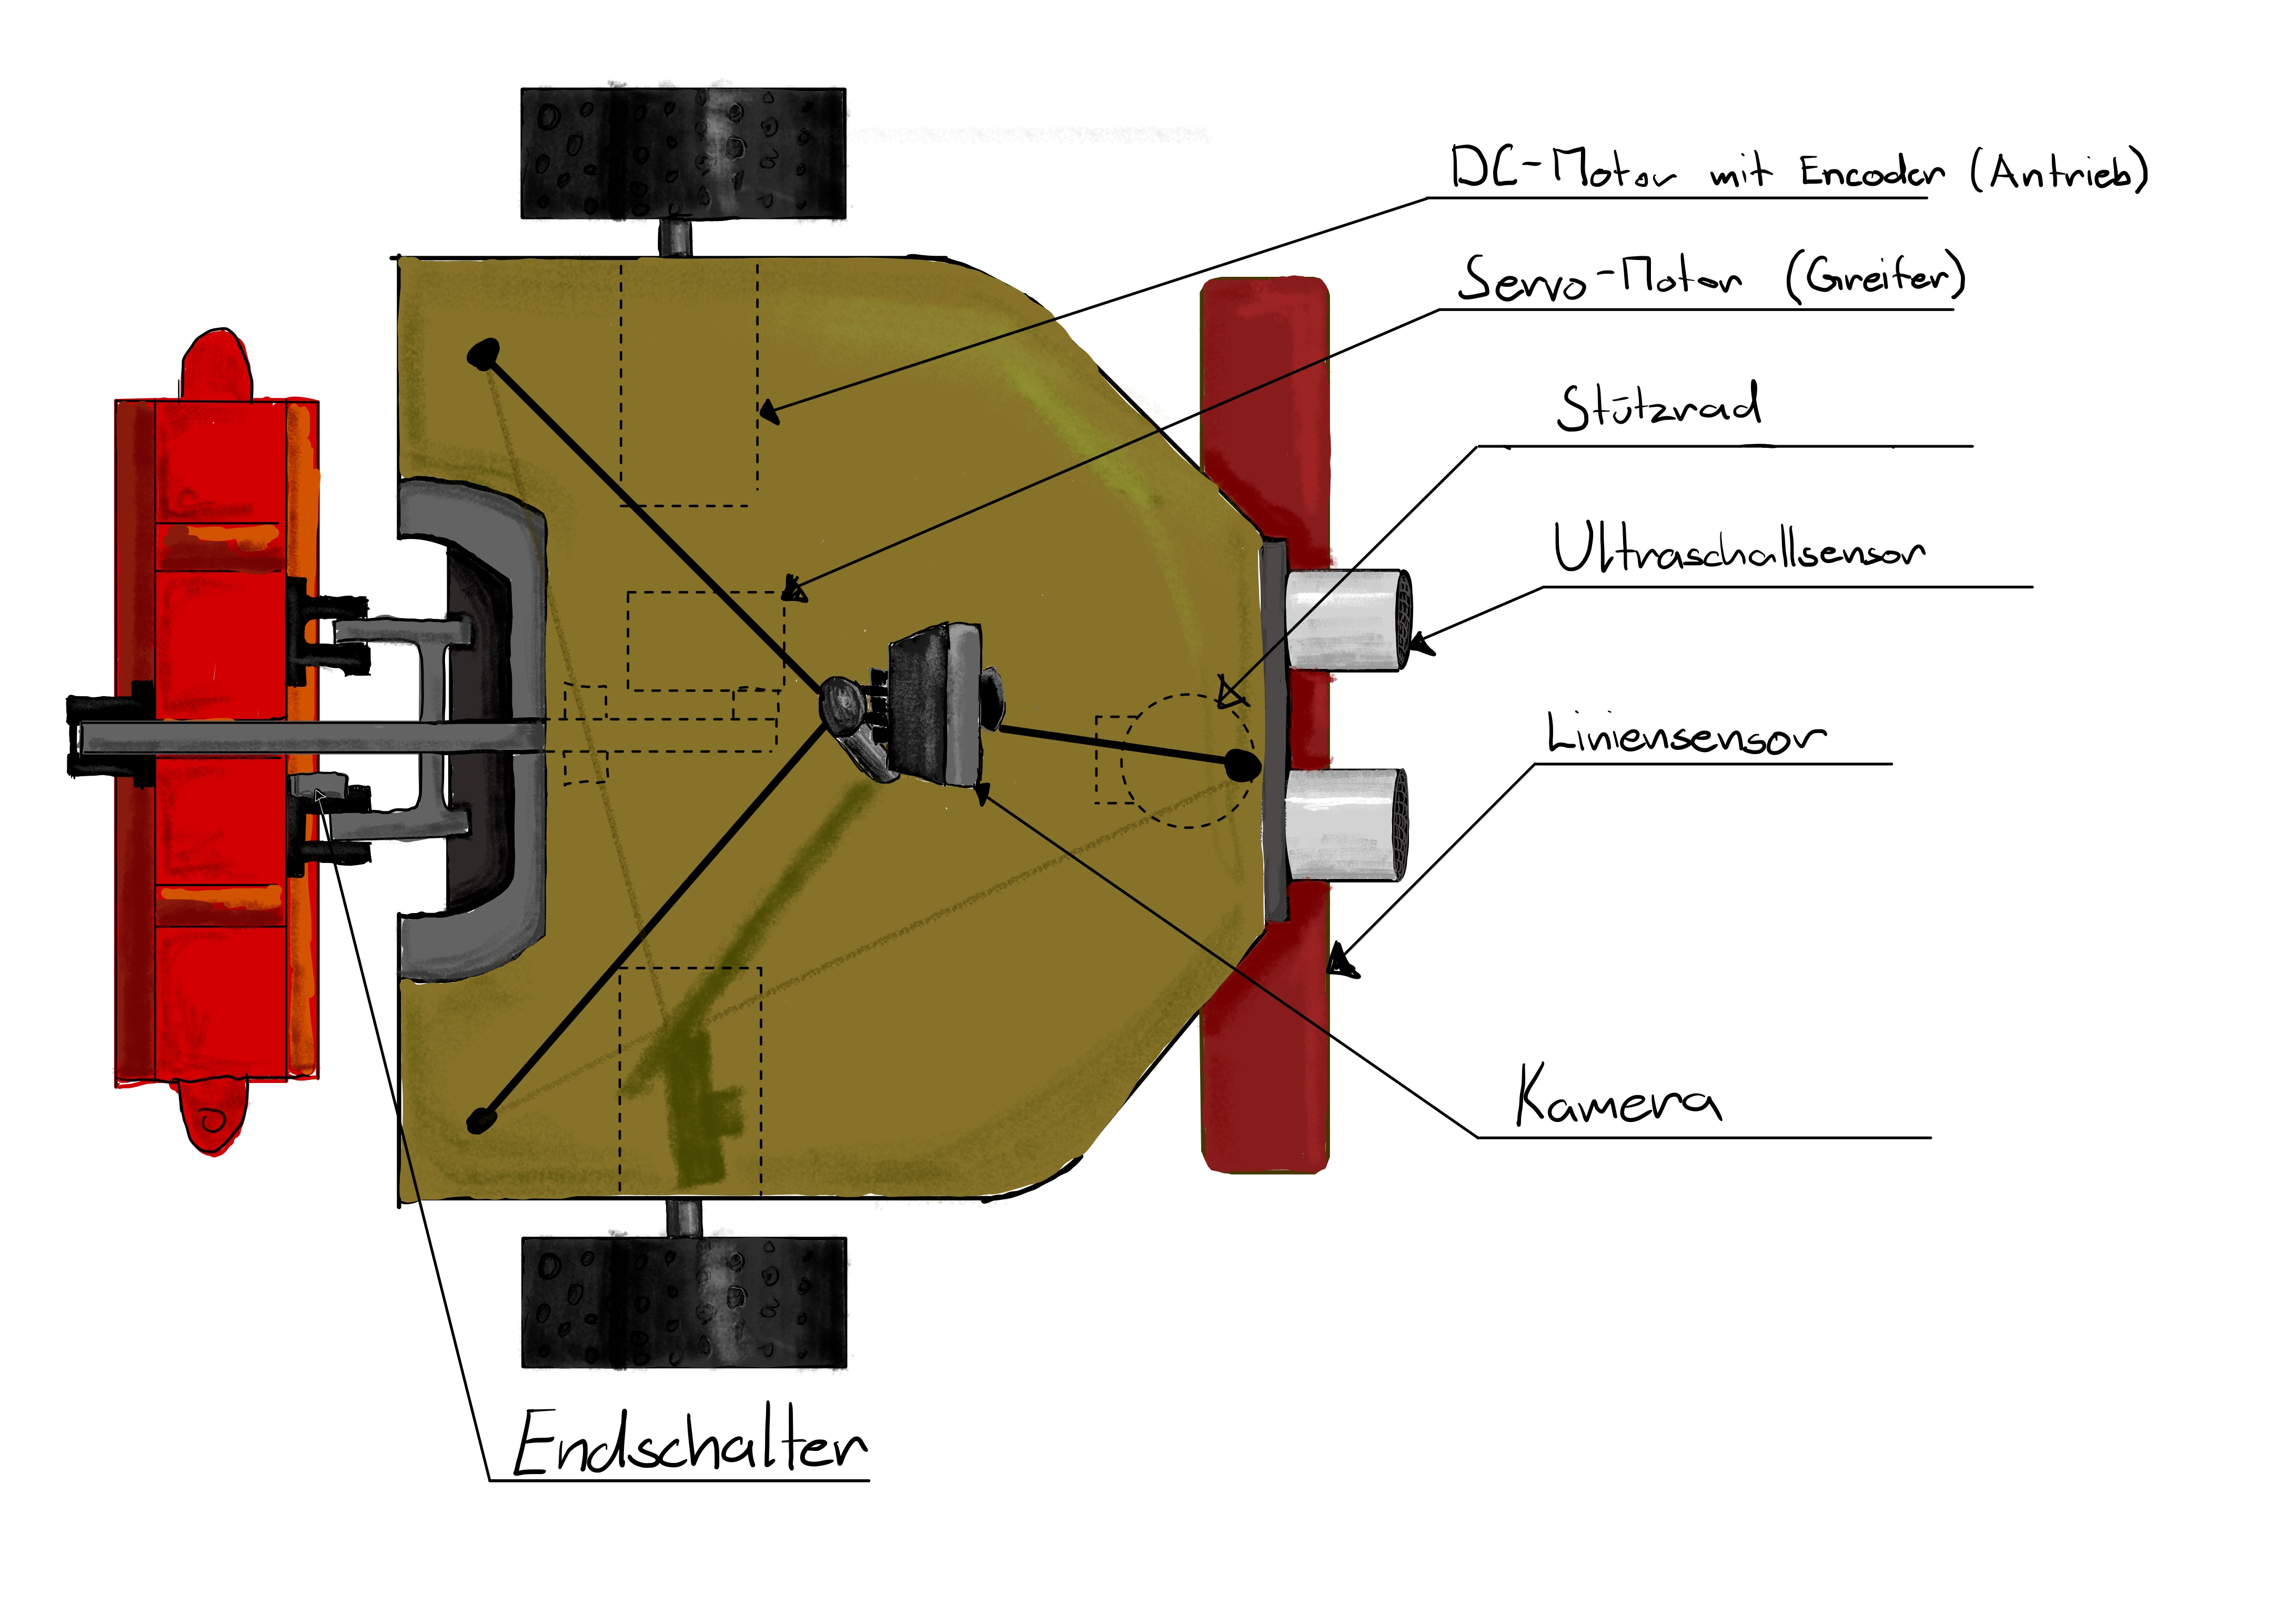
\includegraphics[width=\textwidth]{assets/gesamtkonzept/Skizze-Fahrzeugkonzept-Beschriftet.jpg}
\caption{Komponenten des Roboters}
\label{fig:components}
\end{figure}

Es wurde den Roboter in Abbildung \ref{fig:robo-labeled} gebaut, der die geplanten Komponenten enthält.

Der Servomotor steuert den Greifer an, der die Barriere anheben kann, um sie zu beseitigen. Der Liniensensor sorgt dafür, dass der Roboter nicht von der Linie abkommt und erkennt, wenn er sich auf einem Knoten befindet. Der Ultraschallsensor soll detektieren, wenn der Roboter sich nahe an einer Barriere befindet. Mit der Kamera werden Bilder gemacht, die mit \acrfull{ai} detektiert werden, um herauszufinden, ob sich auf dem Weg Objekte befinden.

\begin{figure}[H]
\centering
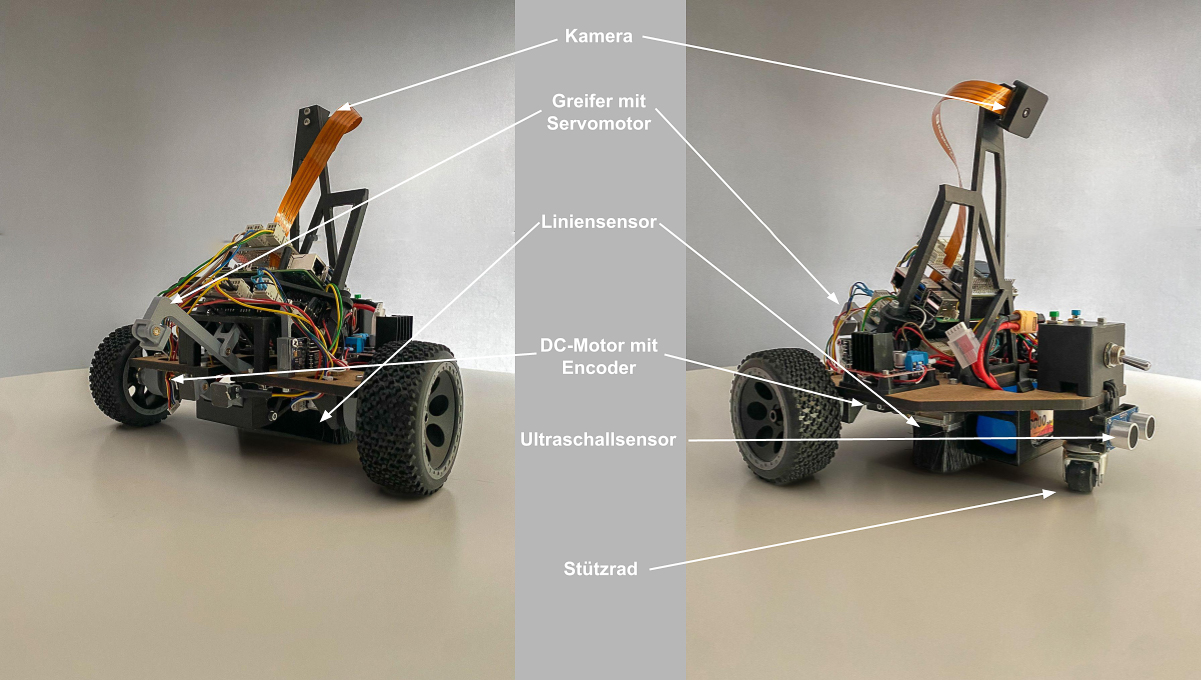
\includegraphics[width=\textwidth]{assets/robo-labeled.jpg}
\caption{Roboter}
\label{fig:robo-labeled}
\end{figure}

\newpage
Abbildung \ref{fig:ablauf} zeigt den geplanten Ablauf auf. Dieses Ablaufdiagramm stammt aus \acrshort{pren1}. Genauere Informationen können aus der angehängten PREN 1 Dokumentation entnommen werden.

\begin{figure}[H]
\centering
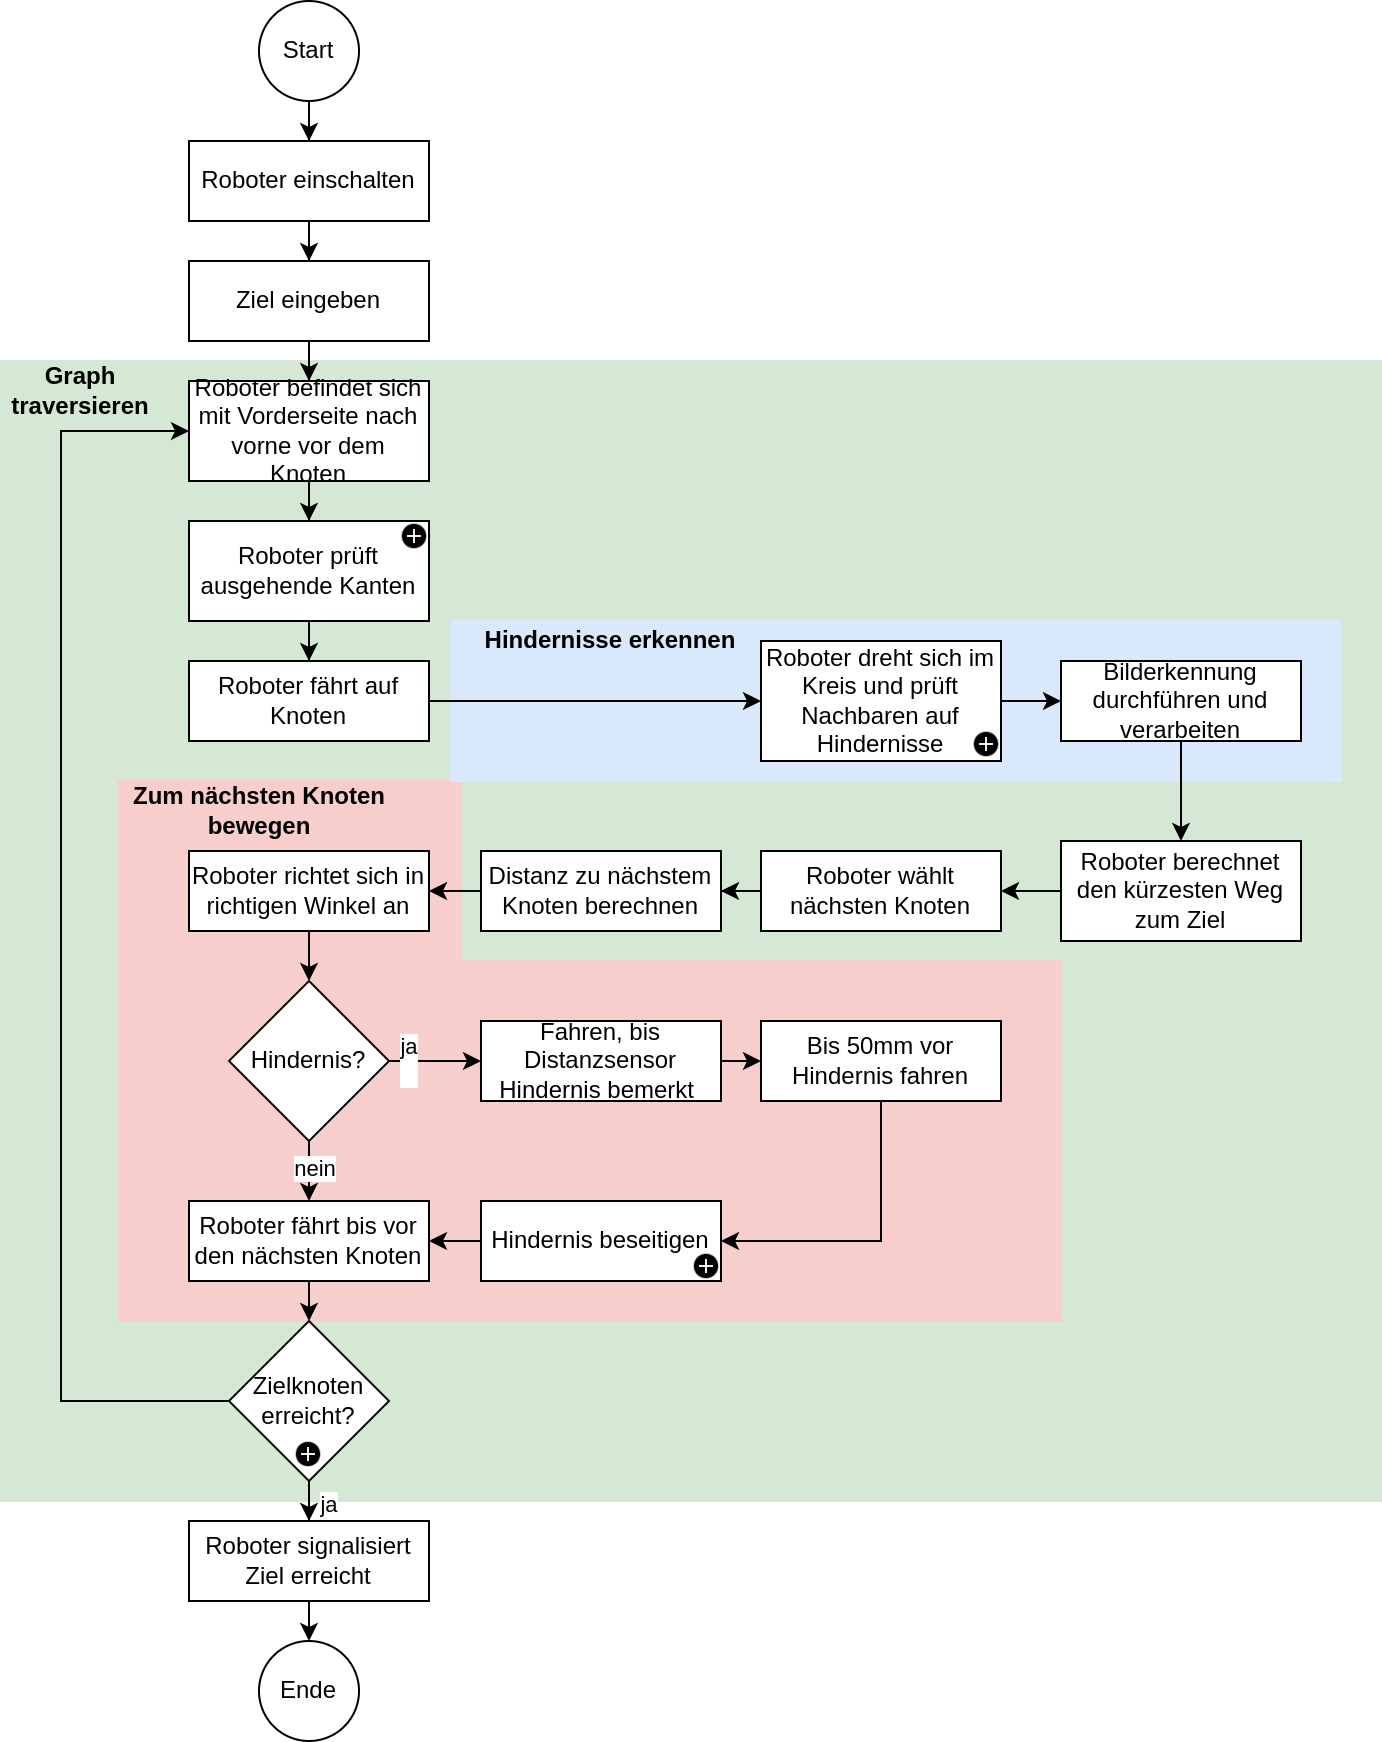
\includegraphics[width=\textwidth]{assets/gesamtkonzept/ablaufdiagramm.png}
\caption{Gesamtkonzept Ablaufdiagramm}
\label{fig:ablauf}
\end{figure}

\newpage
Die einzelnen elektronischen Teile im Roboter bilden das Gesamtsystem ersichtlich auf Abbildung \ref{fig:electro-components}. Dieses sorgt dafür, dass sich der Roboter wie geplant autonom fortbewegen kann.  Die Grafik ist in Elemente der Navigation und solche der Steuerung unterteilt.

Das PCBA ist die zentrale Verbindung. Der TinyK22 liest den Ultraschall, Liniensensor, die Encoder und die Endschalter des Greifers aus und steuert den Servomotor und die Motorentreiber. Der Raspberry Pi und der TinyK22 kommunizieren über UART. Der Raspberry Pi steuert die Kamera an und liest den Startknopf und den Zielauswahlknopf an und zeigt auf dem Display das gewählte Ziel und die Zeit an, die seit dem Start vergangen ist.


\begin{figure}[H]
\centering
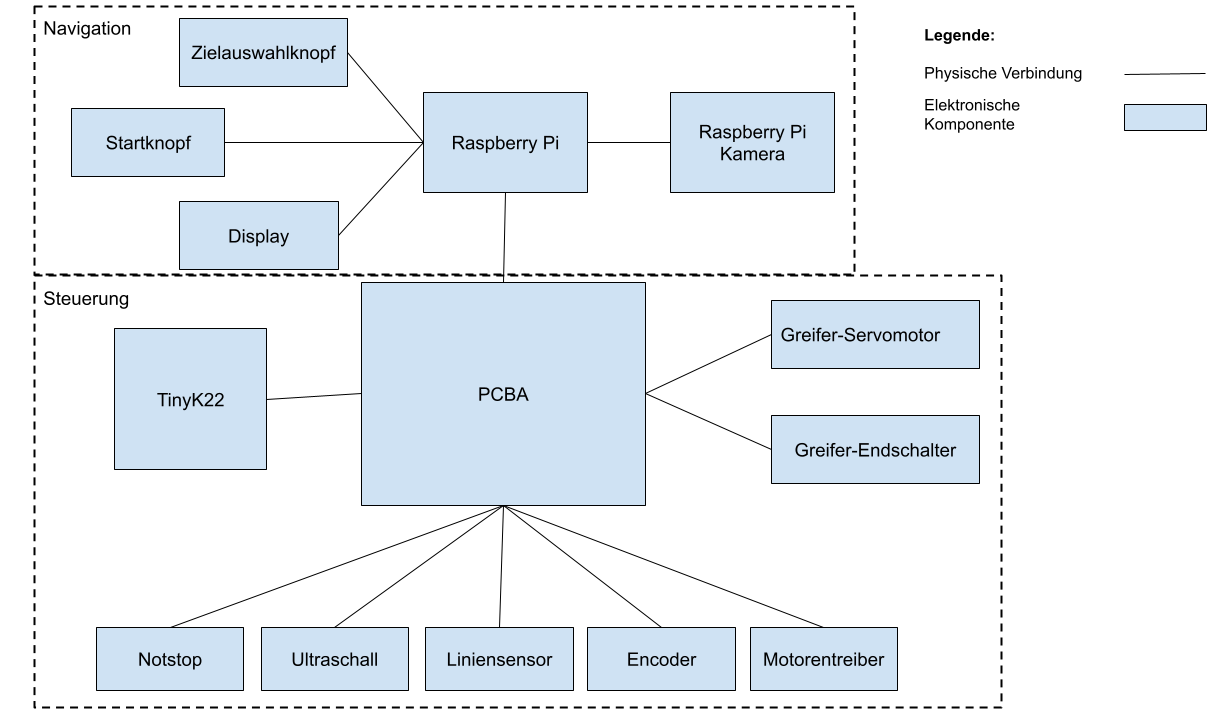
\includegraphics[width=\textwidth]{assets/gesamtkonzept/electronics.png}
\caption{Elektronische Komponenten des Roboters}
\label{fig:electro-components}
\end{figure} 

\newpage

\subsection{Mechanische Komponenten}
\label{Mechanische Komponenten}

Im nachfolgenden Kapitel wird auf die Konstruktion der mechanischen Komponenten eingegangen. Alle Konstruktionsbauteile, bis auf die Grundplatte, wurden im \acrfull{fmd} Verfahren aus \acrfull{pla} gedruckt. Zum Verschrauben der verschiedenen Bauteilen wurden M3 Gewindeeinsätze verwendet.

\subsubsection{Fahrwerk konstruieren}
\label{Fahrwerk konstruieren}

 Das Konzept für das Fahrwerk und die Grundplatte werden analog zum Konzept aus \acrshort{pren1} umgesetzt. Am Fahrwerk werden gegenüber des Prototyps aus \acrshort{pren1} einzig der Motorflansch und der Lenkrollenhalter angepasst. 
 Beim Prototyp in PREN 1 hat sich gezeigt, dass eine reine Presspassung für die Befestigung der Lenkrolle im Lenkrollenhalter aus \acrshort{pla} nicht ausreichend ist. Aus diesem Grund wird die Lenkrolle jetzt mithilfe eines M4 Gewindestifts geklemmt, wie gezeigt auf Abbildung \ref{fig: Lenkrollenhalter V2}.

\begin{figure}[H]
\centering
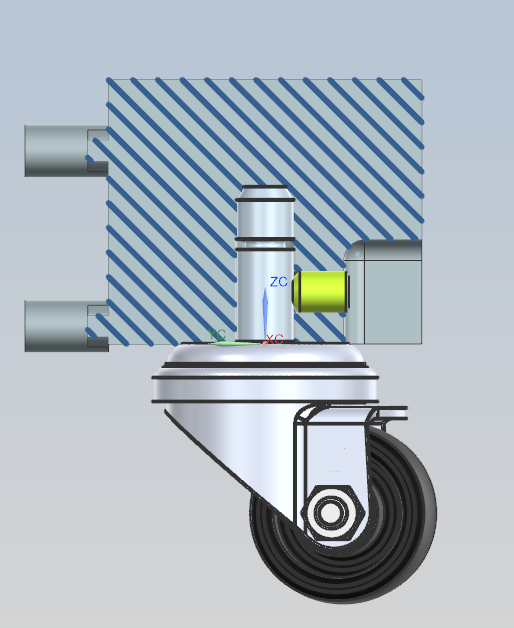
\includegraphics[width=5cm]{assets/MT/Lenkrollenhalter V2.png}
\caption{Lenkrollenhalter V2}
\label{fig: Lenkrollenhalter V2}
\end{figure}

Der Motorflansch wird für den finalen Roboter leicht verstärkt. In Abbildung \ref{fig: Motorflansch V1/V2} ist in gelb die erste Version des Motorflansches ersichtlich, wie er in PREN 1 verbaut wurde. Blau eingefärbt ist die finale Version des Flansches mit einer Verstrebung. Auf Abbildung \ref{fig: Motorentest} wird die Konstruktion am Roboter gezeigt.

\begin{figure}[H]
\centering
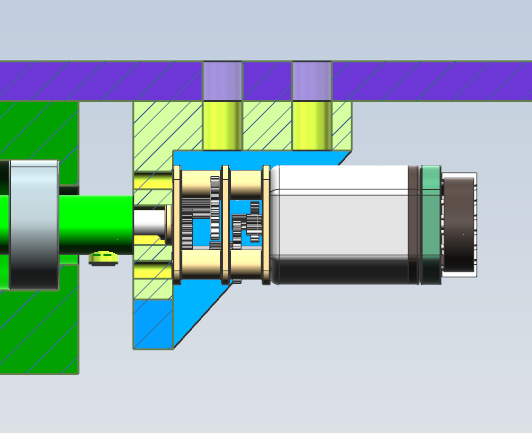
\includegraphics[width=5cm]{assets/MT/Motorflansch Vergleich.png}
\caption{Motorflansch V1/V2}
\label{fig: Motorflansch V1/V2}
\end{figure}

\subsubsection{Montage der Elektronischen Komponenten}
\label{Montage der Elektronischen Komponenten}


Die elektronischen Komponenten wie DC/DC-Konverter, Motortreiber oder Raspberry Pi werden nicht direkt auf die Grundplatte montiert, sondern auf Trägern, welche anschliessend auf die Grundplatte geschraubt werden. Die Träger sind auf der Abbildung \ref{fig: Träger für elektronische Komponenten} in schwarz sichtbar; es ist das schwarze \acrfull{pla} Gerüst unter dem grünen Raspberry Pi. Sie werden so konstruiert, dass die Kabel zwischen Träger und Bauteilen geführt werden können. 
Dieser Aufbau hat in der frühen Testphase den Vorteil, dass alle elektronischen Komponenten provisorisch platziert werden können, ohne einen Kurzschluss zu riskieren. 

\begin{figure}[H]
\centering
\includegraphics[width=5cm]{assets/MT/Träger El Komponenten.jpg}
\caption{Träger für elektronische Komponenten werden zur Kabelführung verwendet}
\label{fig: Träger für elektronische Komponenten}
\end{figure}

\subsubsection{Batteriefach konstruieren}
\label{Batteriefach konstruieren}

Das Batteriefach wird so konstruiert, dass sich die Batterie für die Lagerung jederzeit entfernen lässt. Dafür wird ein Click-Verschluss verwendet. Das Batteriefach wird von unten in die Grundplatte geschoben bis es einrastet. Zum Herausnehmen der Batterie müssen nur die Haken gedrückt werden und das Batteriefach kann ausgefahren werden. Um die Funktion problemlos zu gewährleisten, dürfen die Wandstärken nicht zu gross sein. Damit die Festigkeit trotzdem gewährleistet werden kann, wurde die Layerrichtung im 3D Drucker, wie gezeigt in Abbildung \ref{Layerrichtung Batteriefach}, so gewählt, dass die Layer horizontal zur Verschiebung der Hacken angeordnet sind. Auf Grund der Risikoanalyse in Tabelle \ref{table:risks} wurde entschieden, als zusätzliche Vorsichtsmassnahme eine zweite Halterung herzustellen. So kann bei einem Defekt ohne Unterbruch weiter gearbeitet werden.


\begin{figure}[H]
\centering
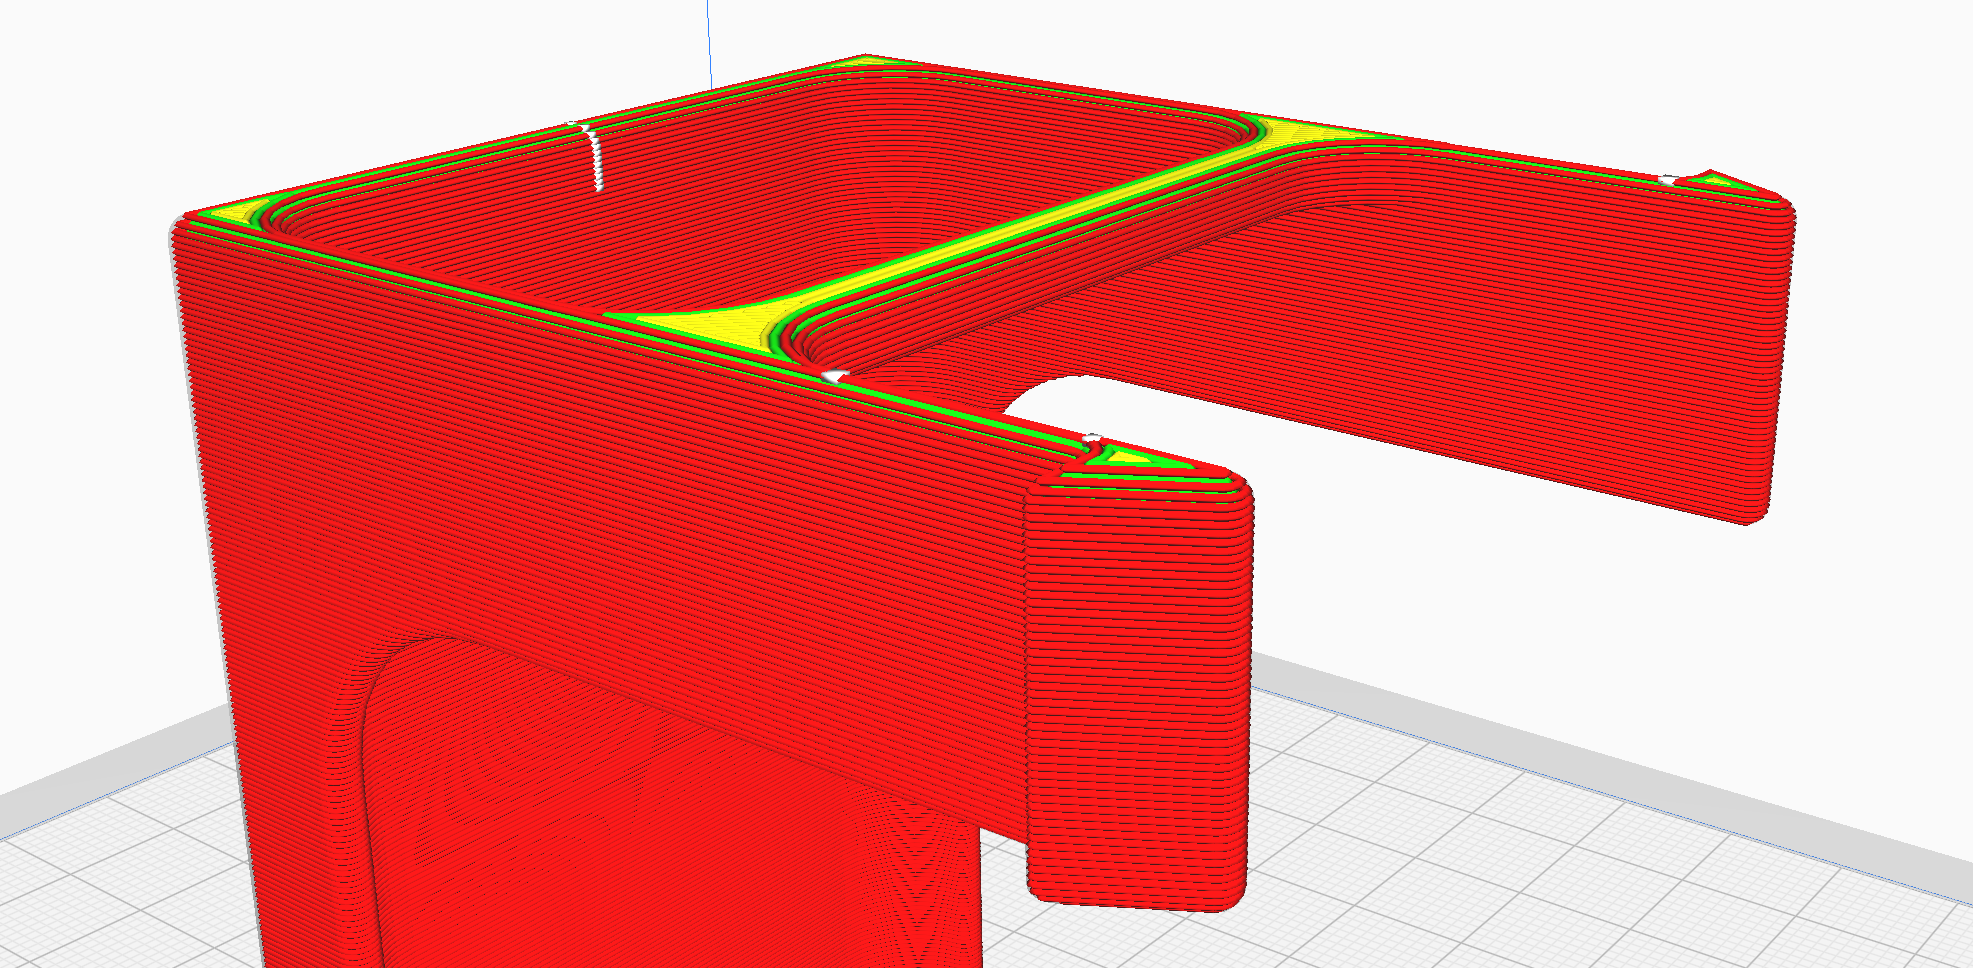
\includegraphics[width=\textwidth]{assets/MT/Layer_Batterie Fach.png}
\caption{FDM Layerrichtung Batteriefach}
\label{Layerrichtung Batteriefach}
\end{figure}

\subsubsection{Greifer konstruieren}
\label{Greifer konstruieren}

Der Klemm- und Hebemechanismus des Greifers sind abhängig von der Federkraft und den Lagerstellen. Dies ist detailliert beschrieben in der Dokumentation von \acrshort{pren1}. Bei der Implementierung des Greifers muss darauf geachtet werden, dass die Lagerstellen nicht verschoben werden. In Abbildung \ref{fig:Greifer im Roboter} \& \ref{fig:Greifer Versuchsaufbau} sind die für die Funktion wichtigsten Masse am Versuchsaufbau und am fertigen Roboter gezeigt. Die für die Haltekraft verantwortliche Feder, sowie alle Haltebacken und Pendelstützen wurden vom Prototyp wiederverwendet. 

\begin{figure}[H]
  \centering
  \begin{minipage}[b]{0.45\textwidth}
    \centering
    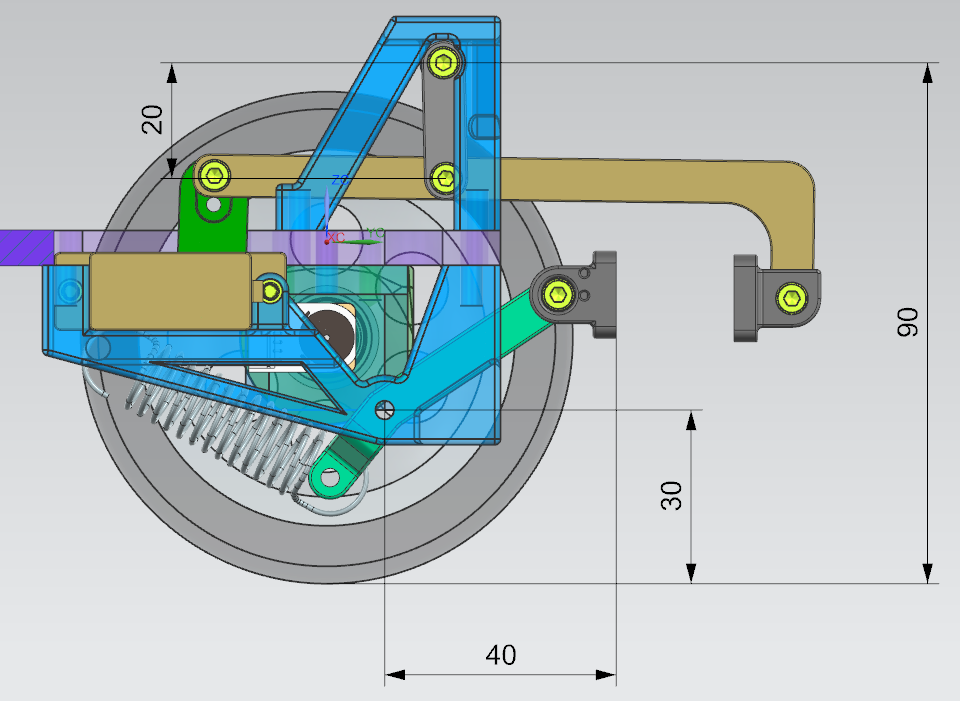
\includegraphics[height=5cm]{assets/MT/Greifer Montiert.png}
    \caption{Greifer im Roboter}
    \label{fig:Greifer im Roboter}
  \end{minipage}
  \hfill
  \begin{minipage}[b]{0.45\textwidth}
    \centering
    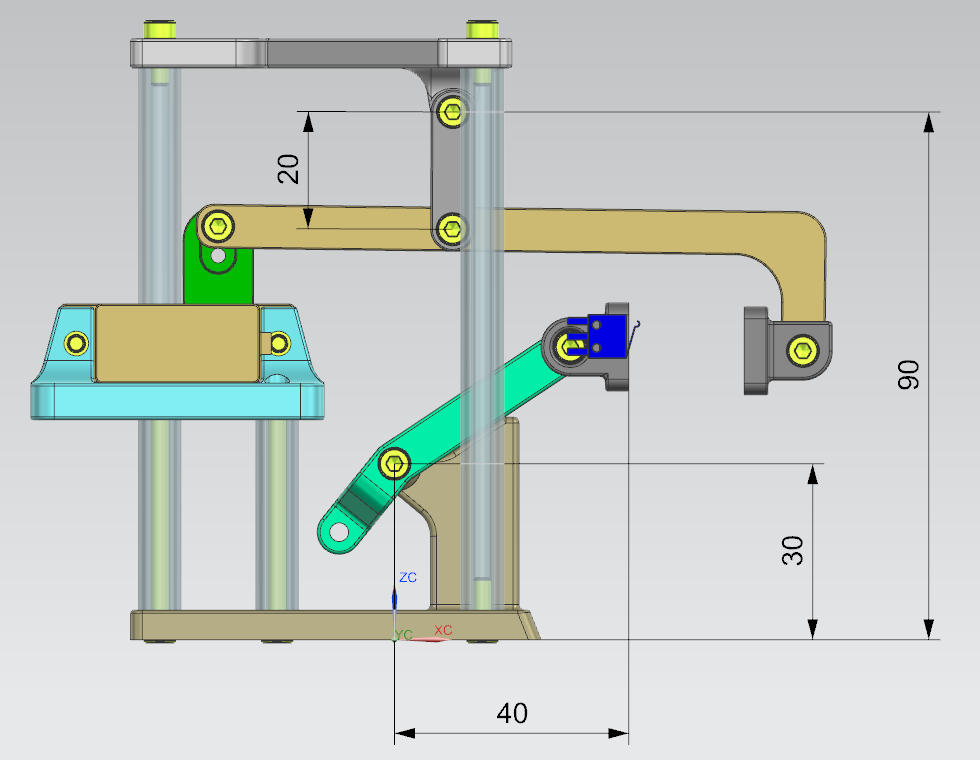
\includegraphics[height=5cm]{assets/MT/Greifer Prototyp.png}
    \caption{Greifer Versuchsaufbau}
    \label{fig:Greifer Versuchsaufbau}
  \end{minipage}
\end{figure}

\newpage

\subsubsection{Halterung Liniensensor}
\label{Halterung Liniensensor}

Der Liniensensor wird mit einer zweiteiligen Halterung befestigt. Auf der inneren Schale, in Abbildung \ref{fig:Schnitt Halterung Liniensensor} blau, ist der Sensor befestigt. Die innere Schale lässt sich verschieben. So kann die Höhe eingestellt werden. Die Fixierung erfolgt mithilfe von zwei Gewindestiften, die in der äusseren Schale befestigt werden und die innere Schale klemmen. 


\begin{figure}[H]
    \centering
    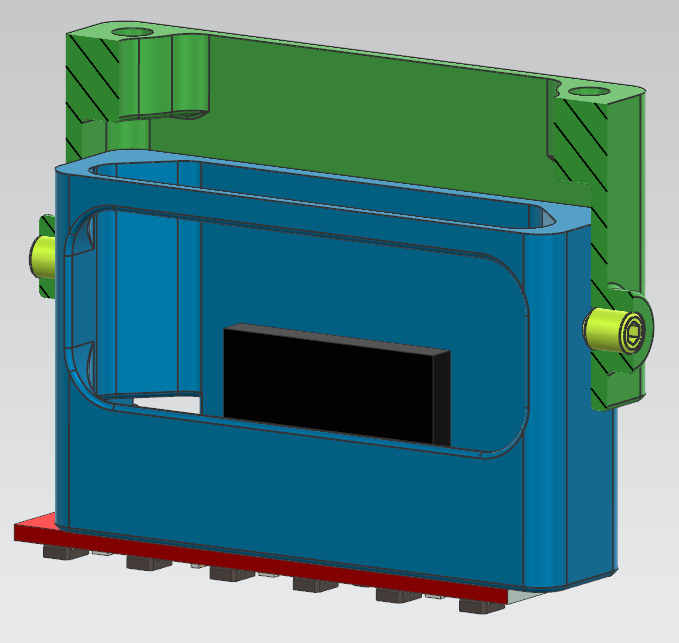
\includegraphics[width=0.75\linewidth]{assets//MT/Sensor Halterung.png}
    \caption{Schnitt Halterung Liniensensor}
    \label{fig:Schnitt Halterung Liniensensor}
\end{figure}


\subsubsection{Abschirmung des Liniensensors}
\label{Abschirmung des Liniensensors}

Um Störungen durch Fremdlicht zu verhindern, wird eine Abdeckung konstruiert, die jegliche Fremdeinstrahlung abschirmt. Als Dichtung wird ein Bürstenband verwendet, wie es üblicherweise bei Schiebetüren zum Einsatz kommt. Die Bürsten werden in einer Halterung eingesteckt und mit einem Gewindestift geklemmt.  Diese Abschirmung war in \acrshort{pren1} noch nicht geplant.


\begin{figure}[H]
 
\end{figure}
\newpage

\begin{figure}[H]
\centering
\begin{minipage}[b]{0.45\textwidth}
  \centering
    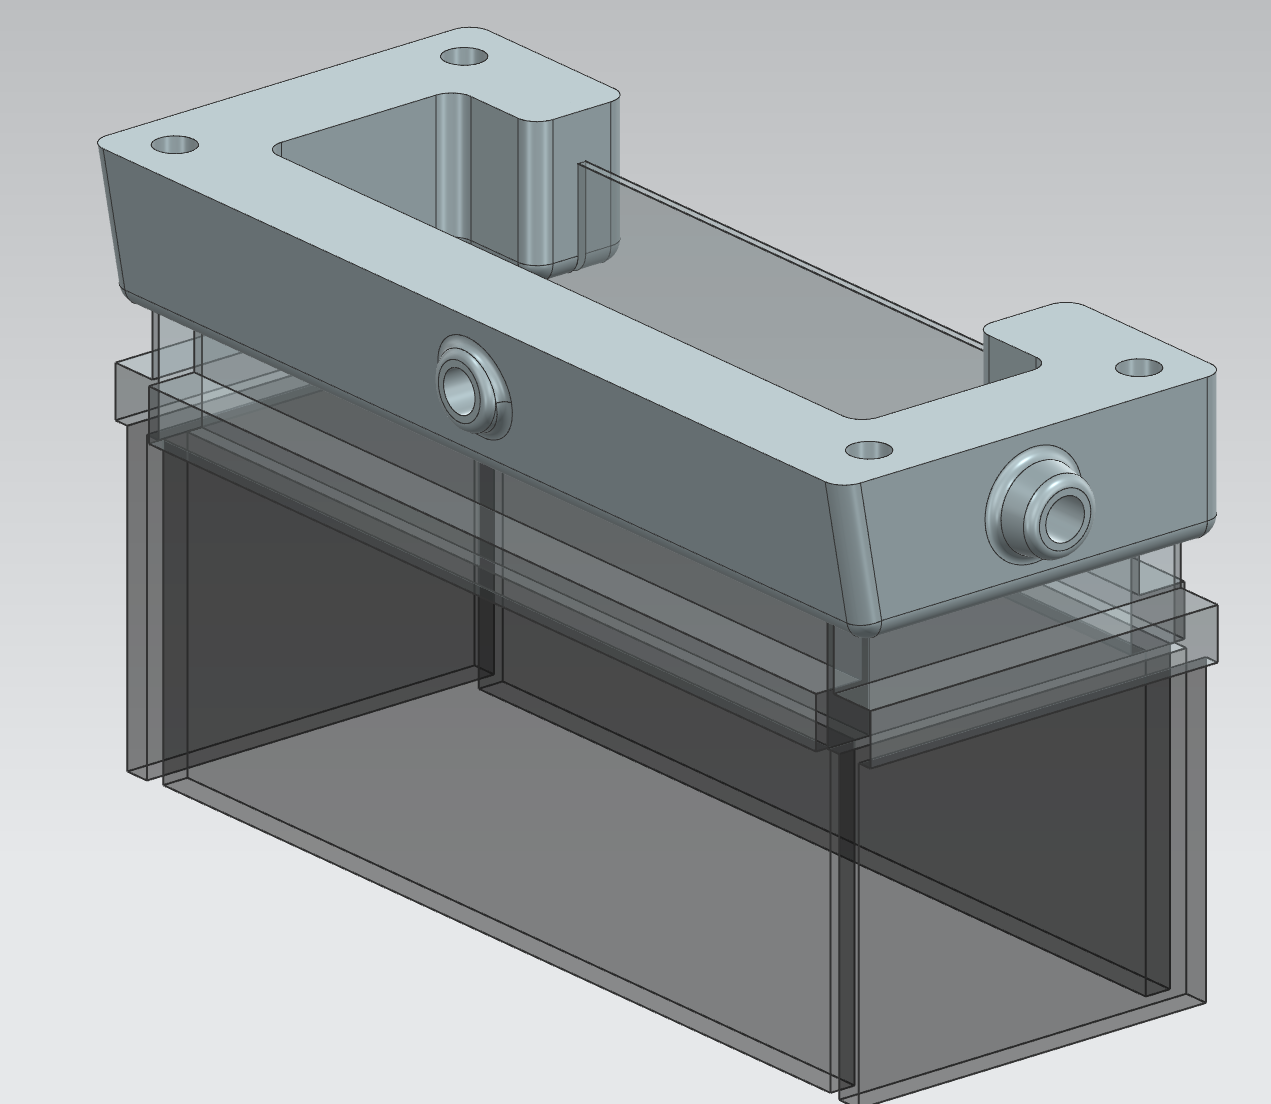
\includegraphics[width=\textwidth]{assets//MT/Sensor Abdeckung.png}
    \caption{Liniensensor Abschirmung}
    \label{fig:Liniensensor Abdeckung}
\end{minipage}
\hspace{0.05\textwidth} % Abstand zwischen den Bildern
\begin{minipage}[b]{0.45\textwidth}
  \centering
  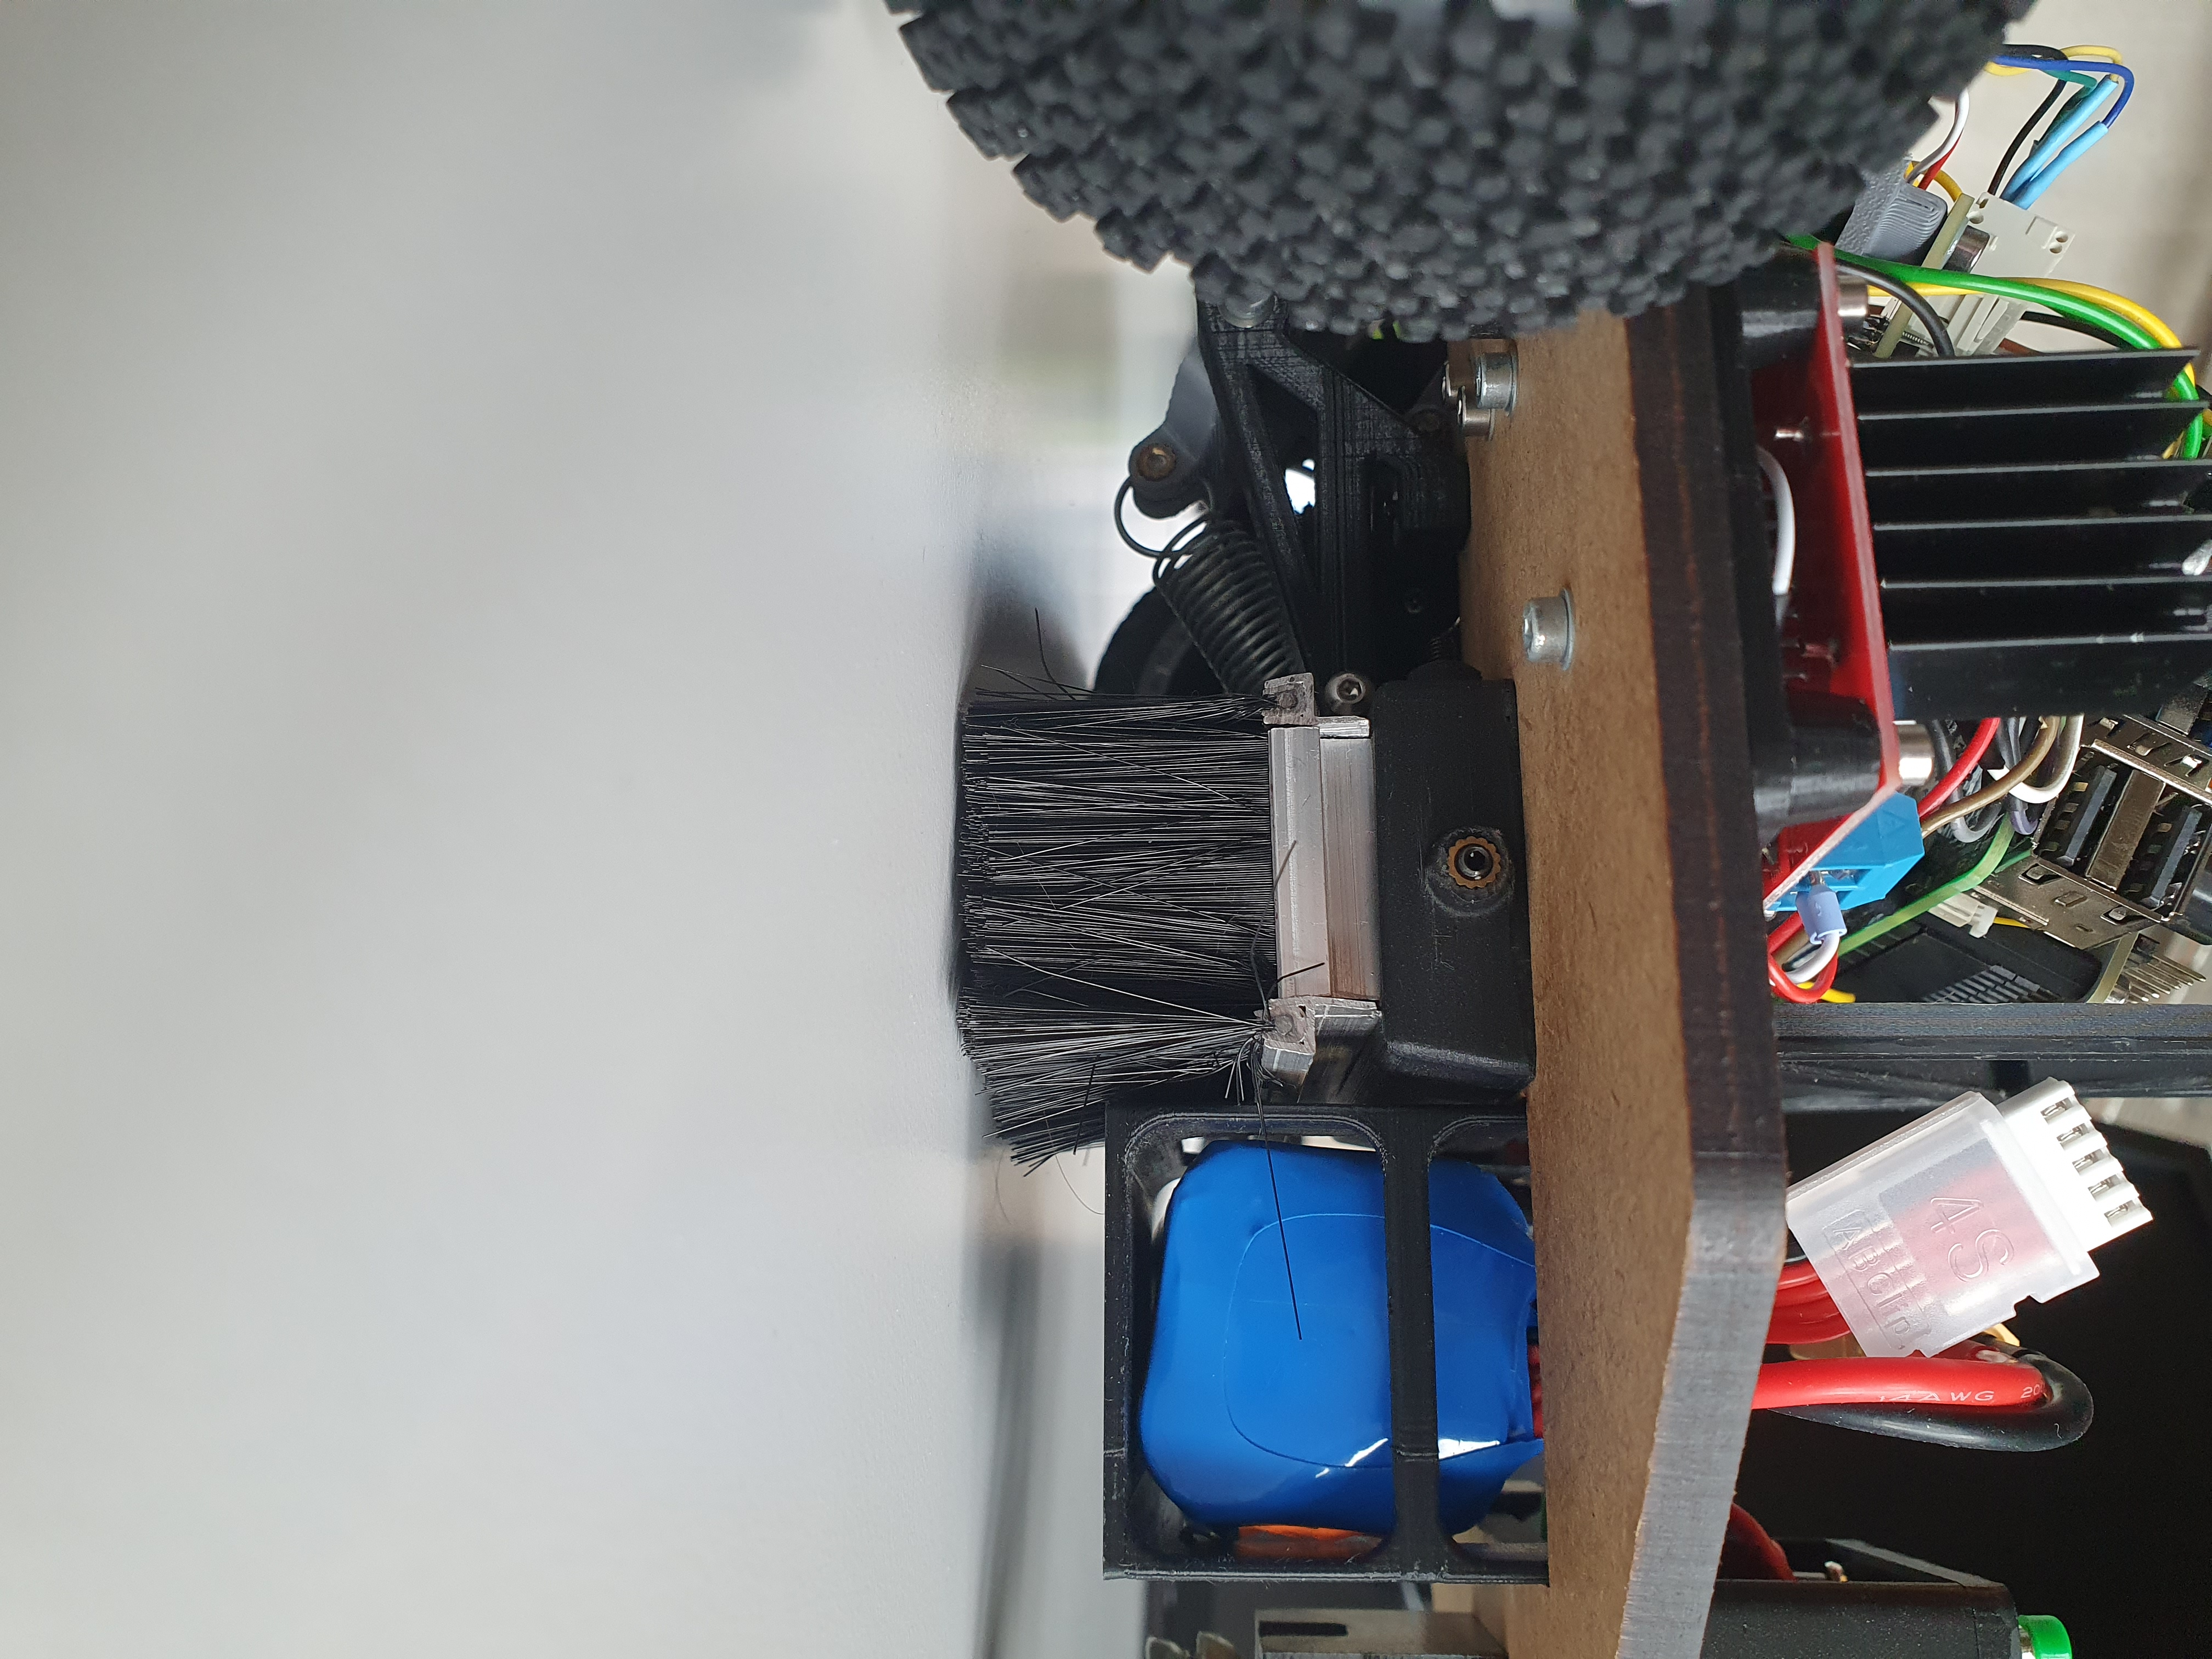
\includegraphics[width=\textwidth, angle=90]{assets/MT/liniensensor-beseli.jpg}
  \caption{Abschirmung am Roboter}
  \label{fig:abschirmung-robi}
\end{minipage}
\end{figure}


\subsubsection{Ultraschall}

Es wird ein Ultraschallsensor montiert. Dieser wird für die Bewältigung der Hindernisse benötigt und ebenfalls dient er als Backup, um Objekte zu erkennen. Falls die Kamera ein Objekte nicht erkennt, dann würde der Ultraschall dieses bemerken, wenn der Roboter sich davor befindet. Das sorgt dafür, dass Kollisionen vermieden werden.

Der Ultraschall wird ganz vorne am Roboter angebracht, auf der Höhe, die optimal ist, um die Barriere zu erkennen. Der Ultraschall misst direkt über den Löchern, die es in der Barriere gibt, so können die Wellen sicher an einer geraden Fläche reflektiert werden. Die Höhe im Vergleich mit einer Barriere ist auf Abbildung \ref{fig:ultraschall-hoehe} gezeigt.

\begin{figure}[H]
\centering
\begin{minipage}[b]{0.45\textwidth}
  \centering
  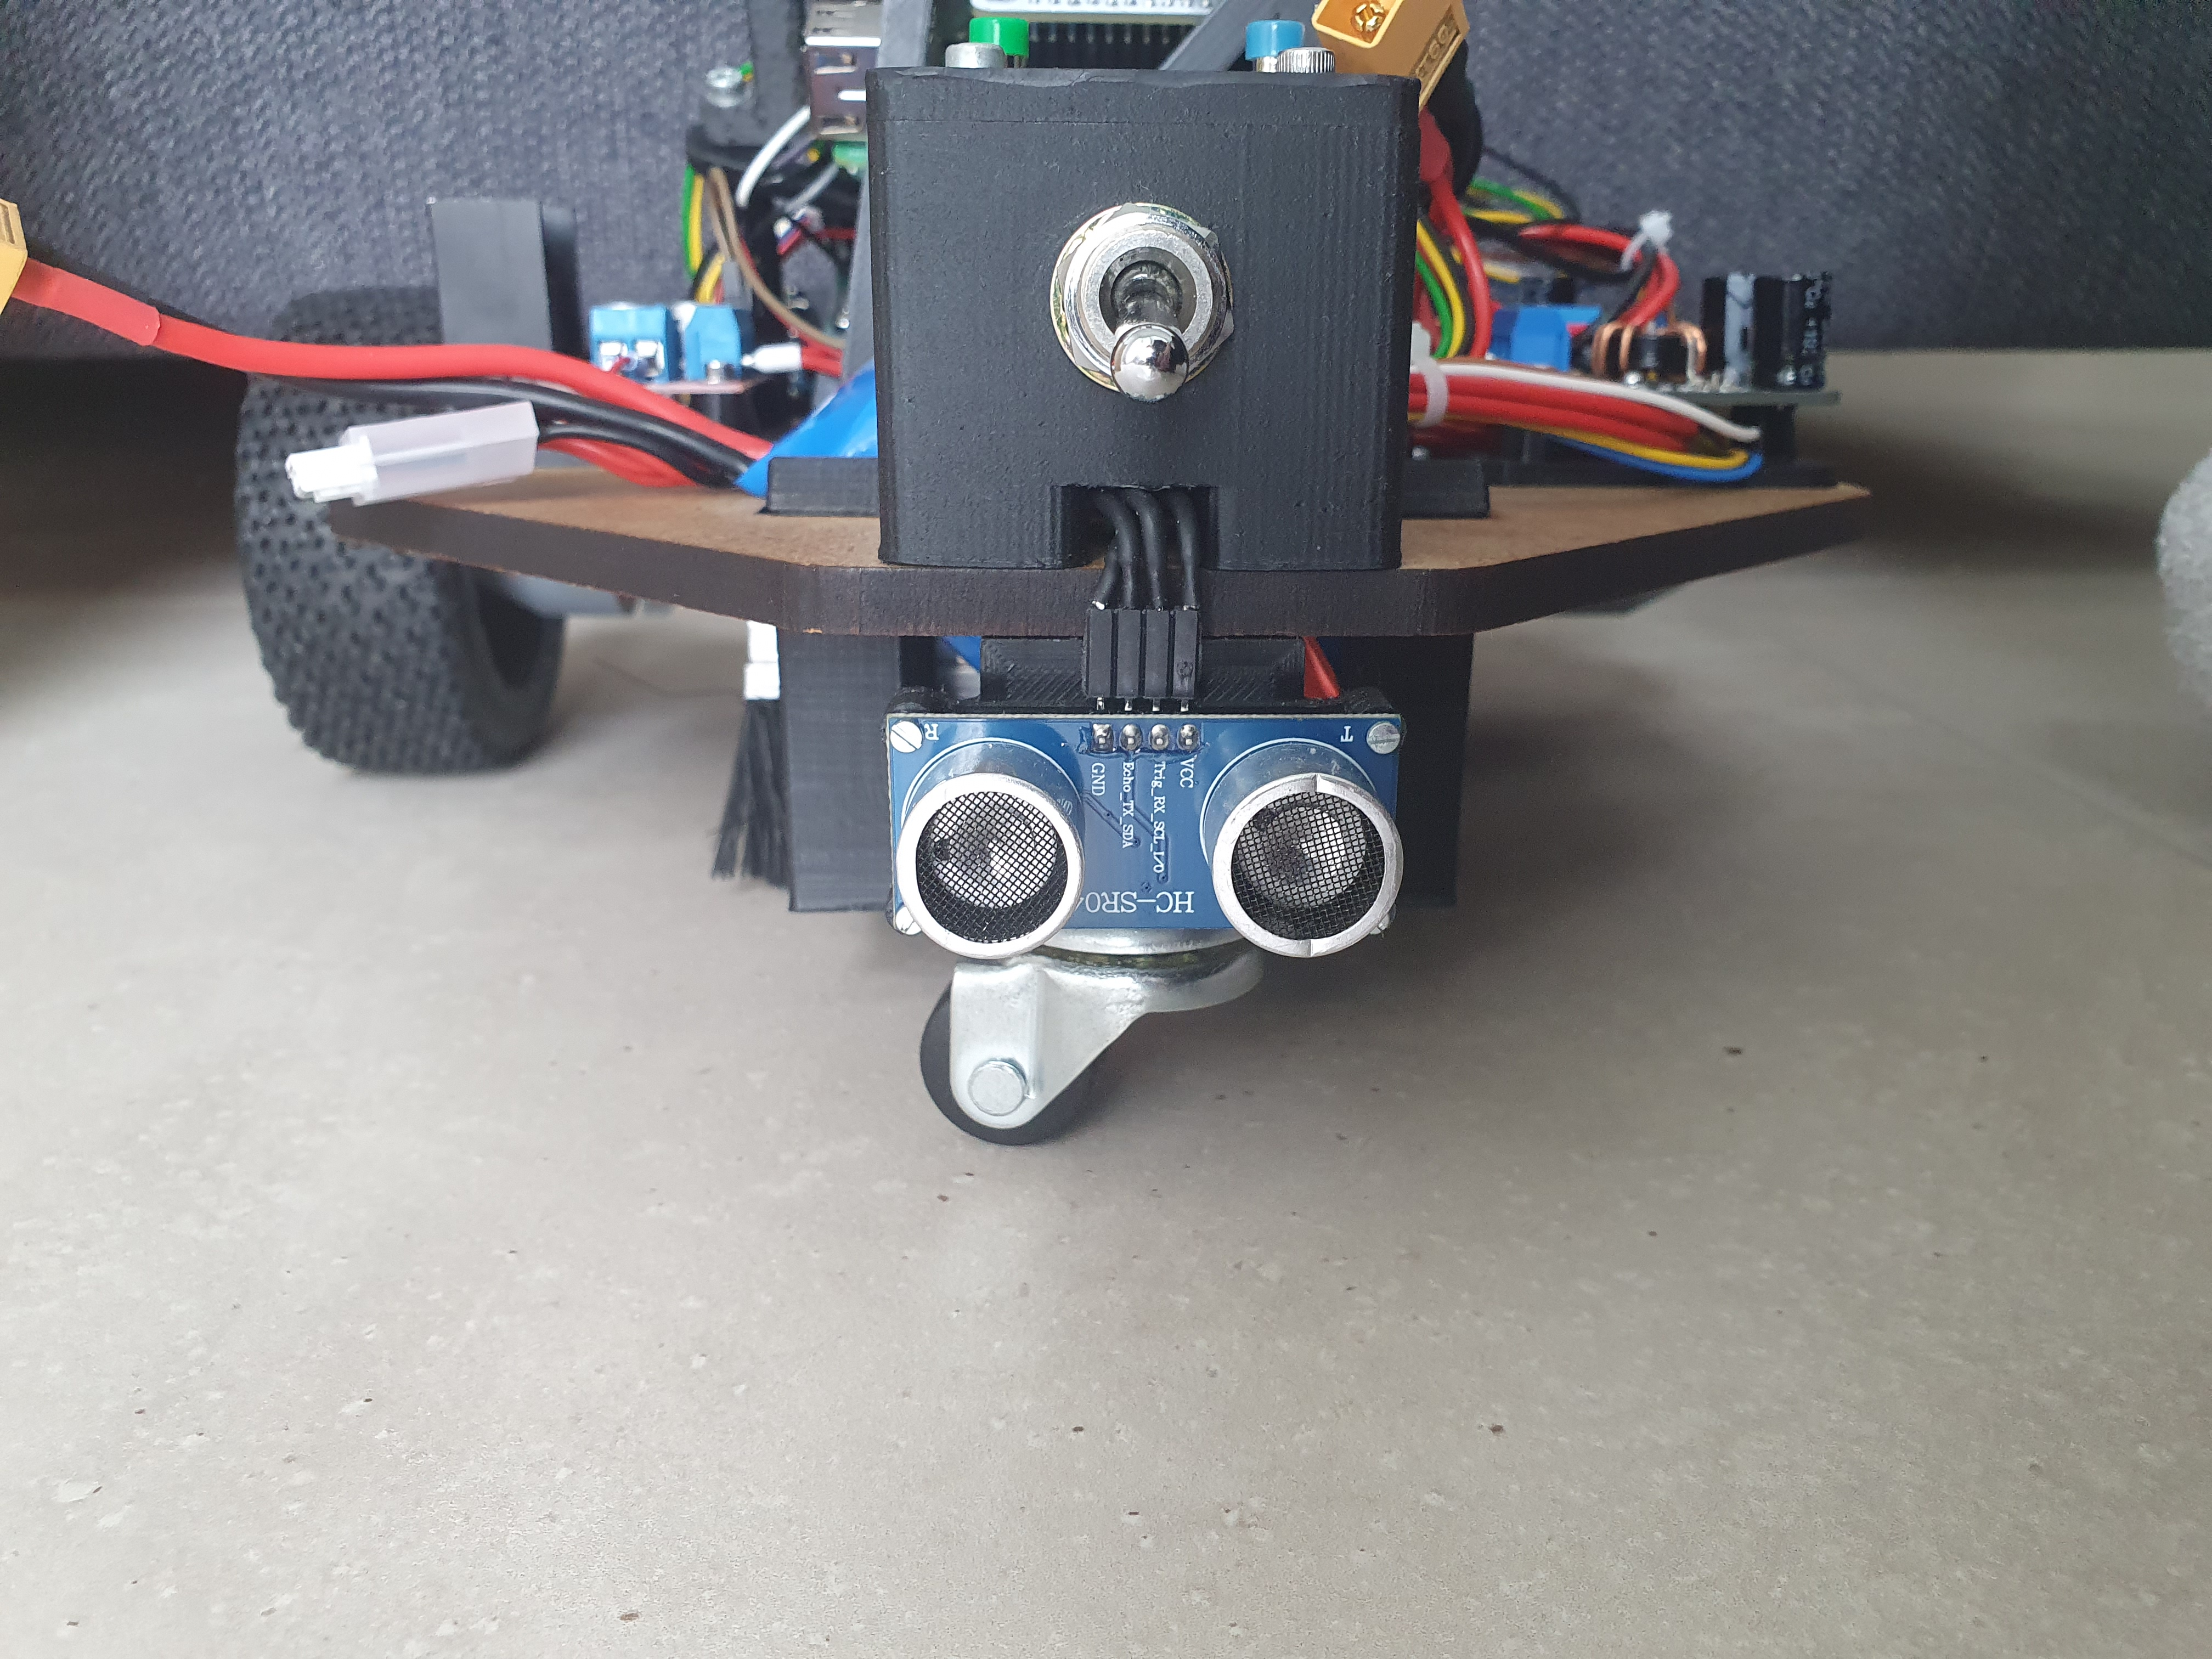
\includegraphics[width=\textwidth]{assets/ET/ultraschall/ultraschall.jpg}
  \caption{Ultraschall am Roboter}
  \label{fig:ultraschall-robi}
\end{minipage}
\hspace{0.05\textwidth} % Abstand zwischen den Bildern
\begin{minipage}[b]{0.45\textwidth}
  \centering
  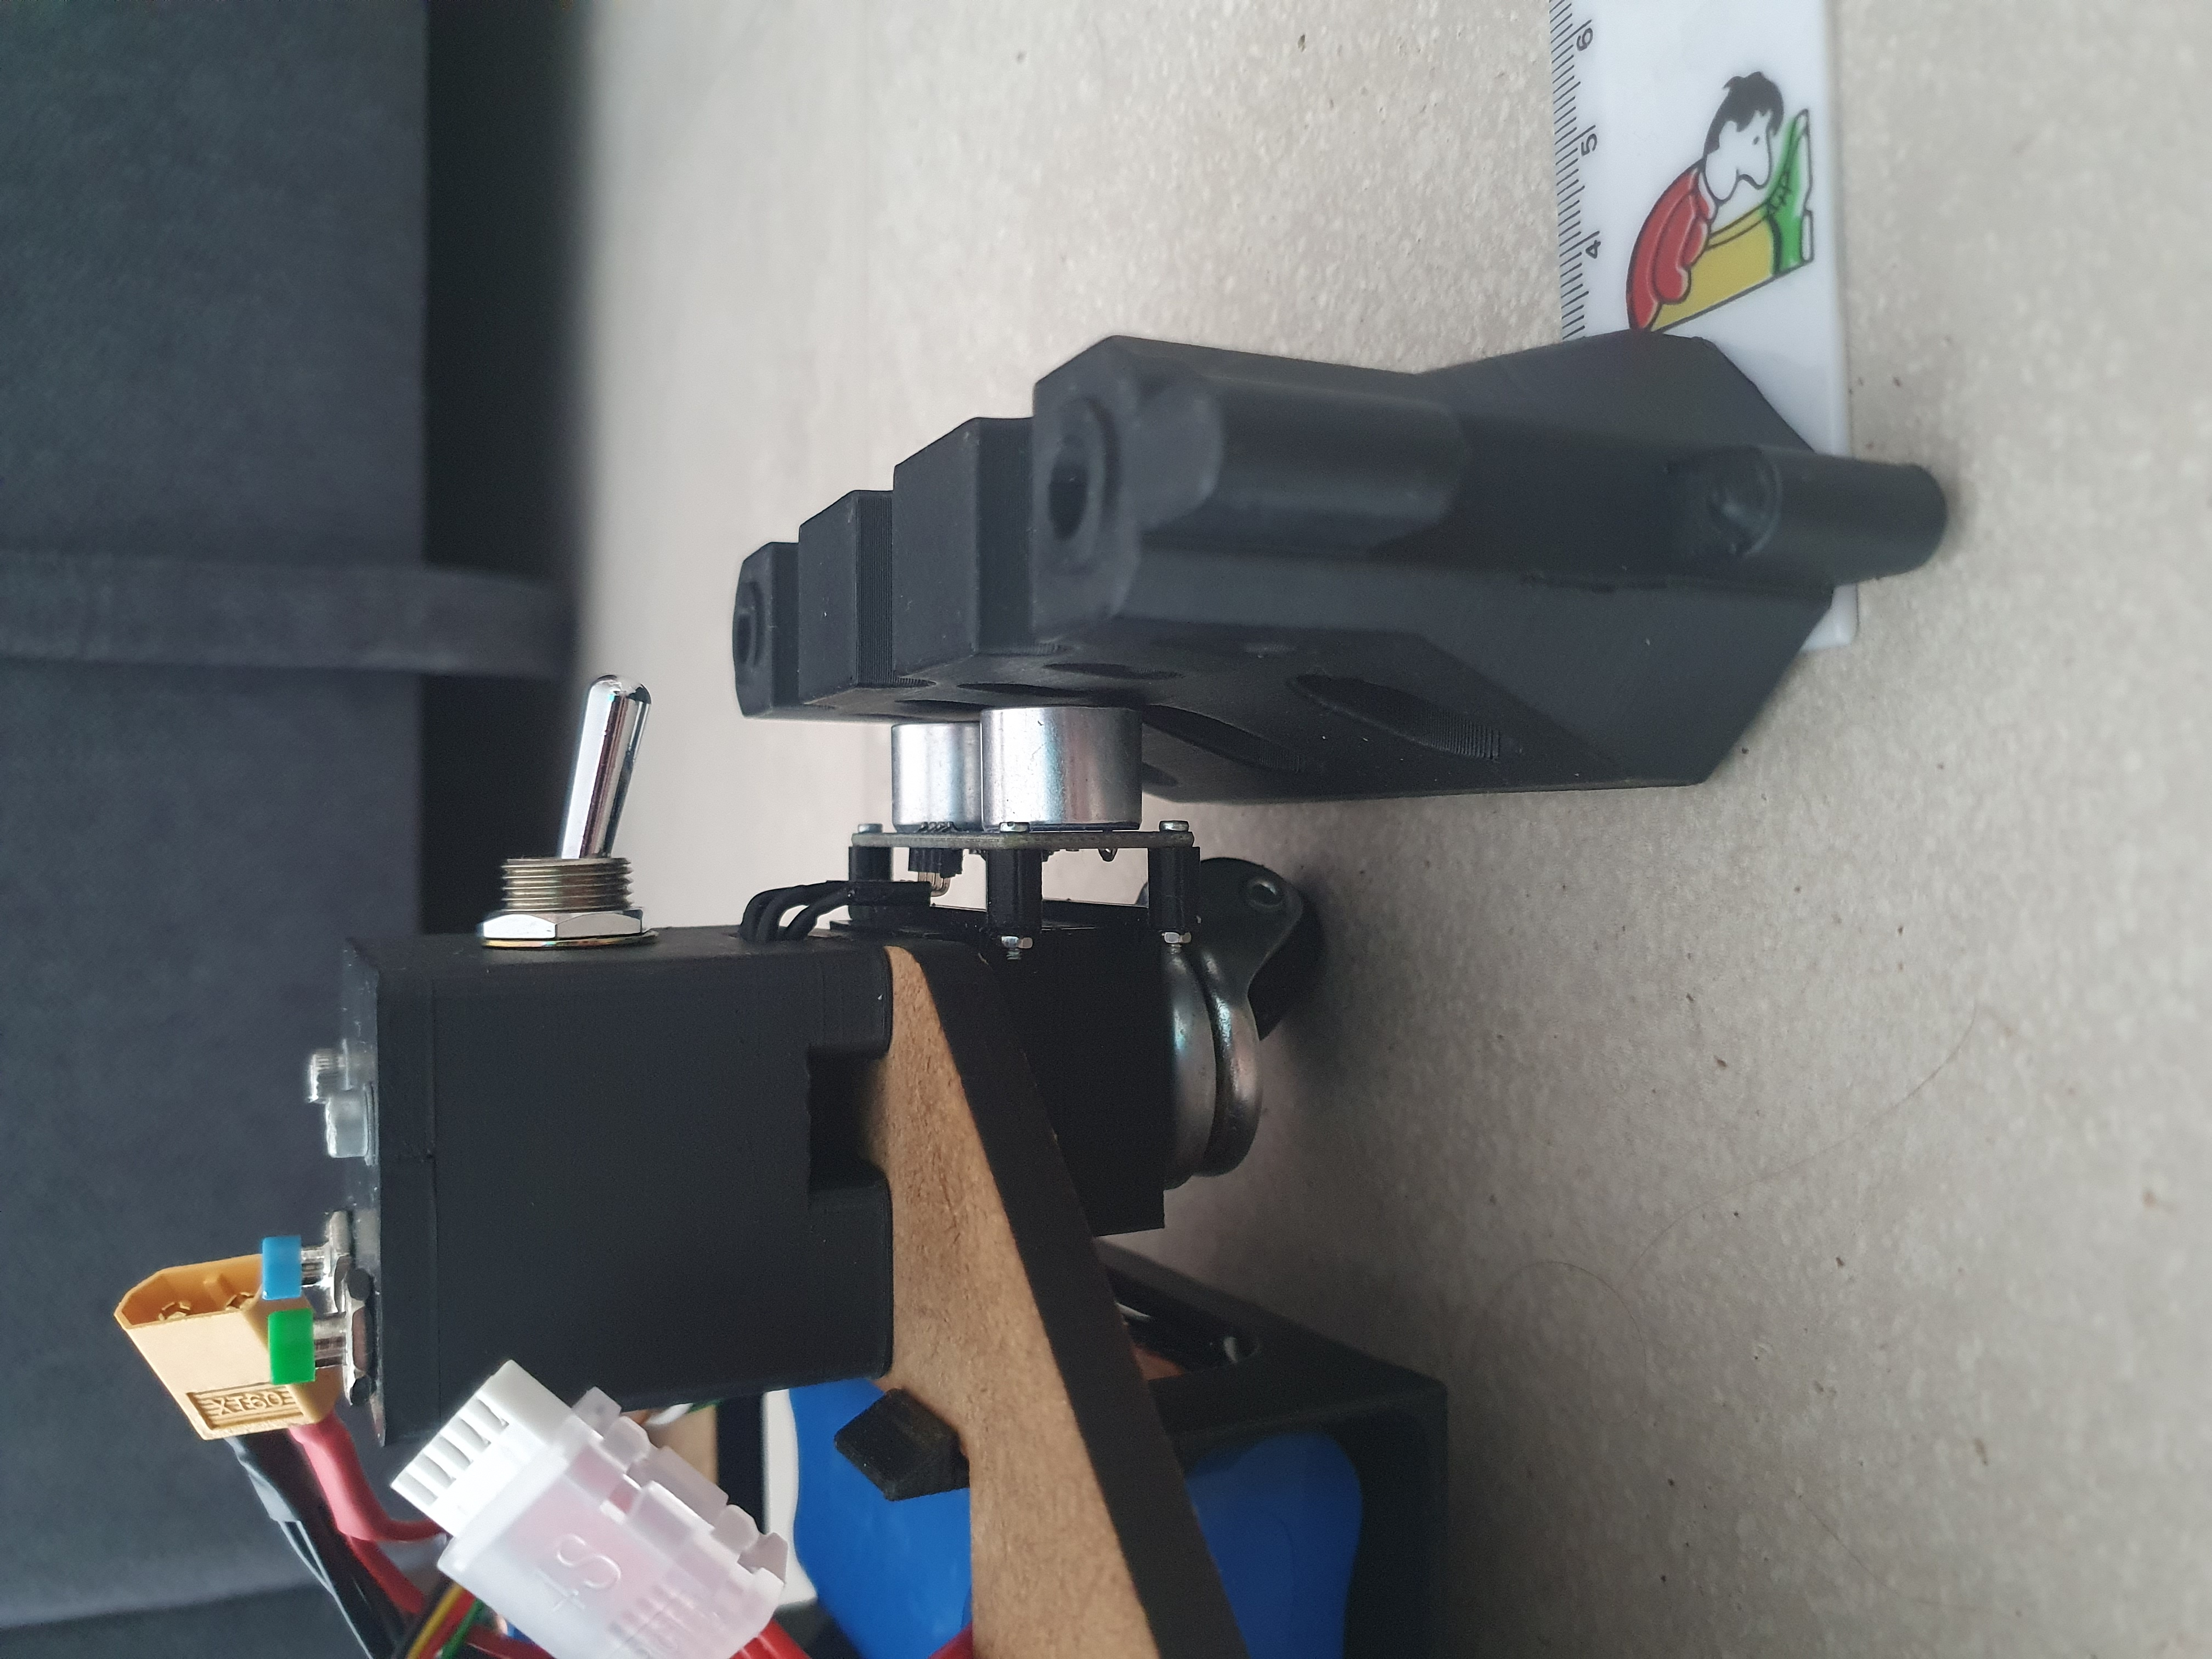
\includegraphics[width=\textwidth, angle=-90]{assets/ET/ultraschall/ultraschall-side.jpg}
  \caption{Ultraschall Höhe}
  \label{fig:ultraschall-hoehe}
\end{minipage}
\end{figure}

Der Ultraschall wurde getestet, indem die Barriere auf einem Massstab verschoben wurde. So konnten die ausgegebenen Werte mit den Werten, die auf dem Massstab ersichtlich waren, verglichen werden. Objekte können auf \pm 1cm exakt erkannt werden.

\begin{figure}[H]
    \centering
    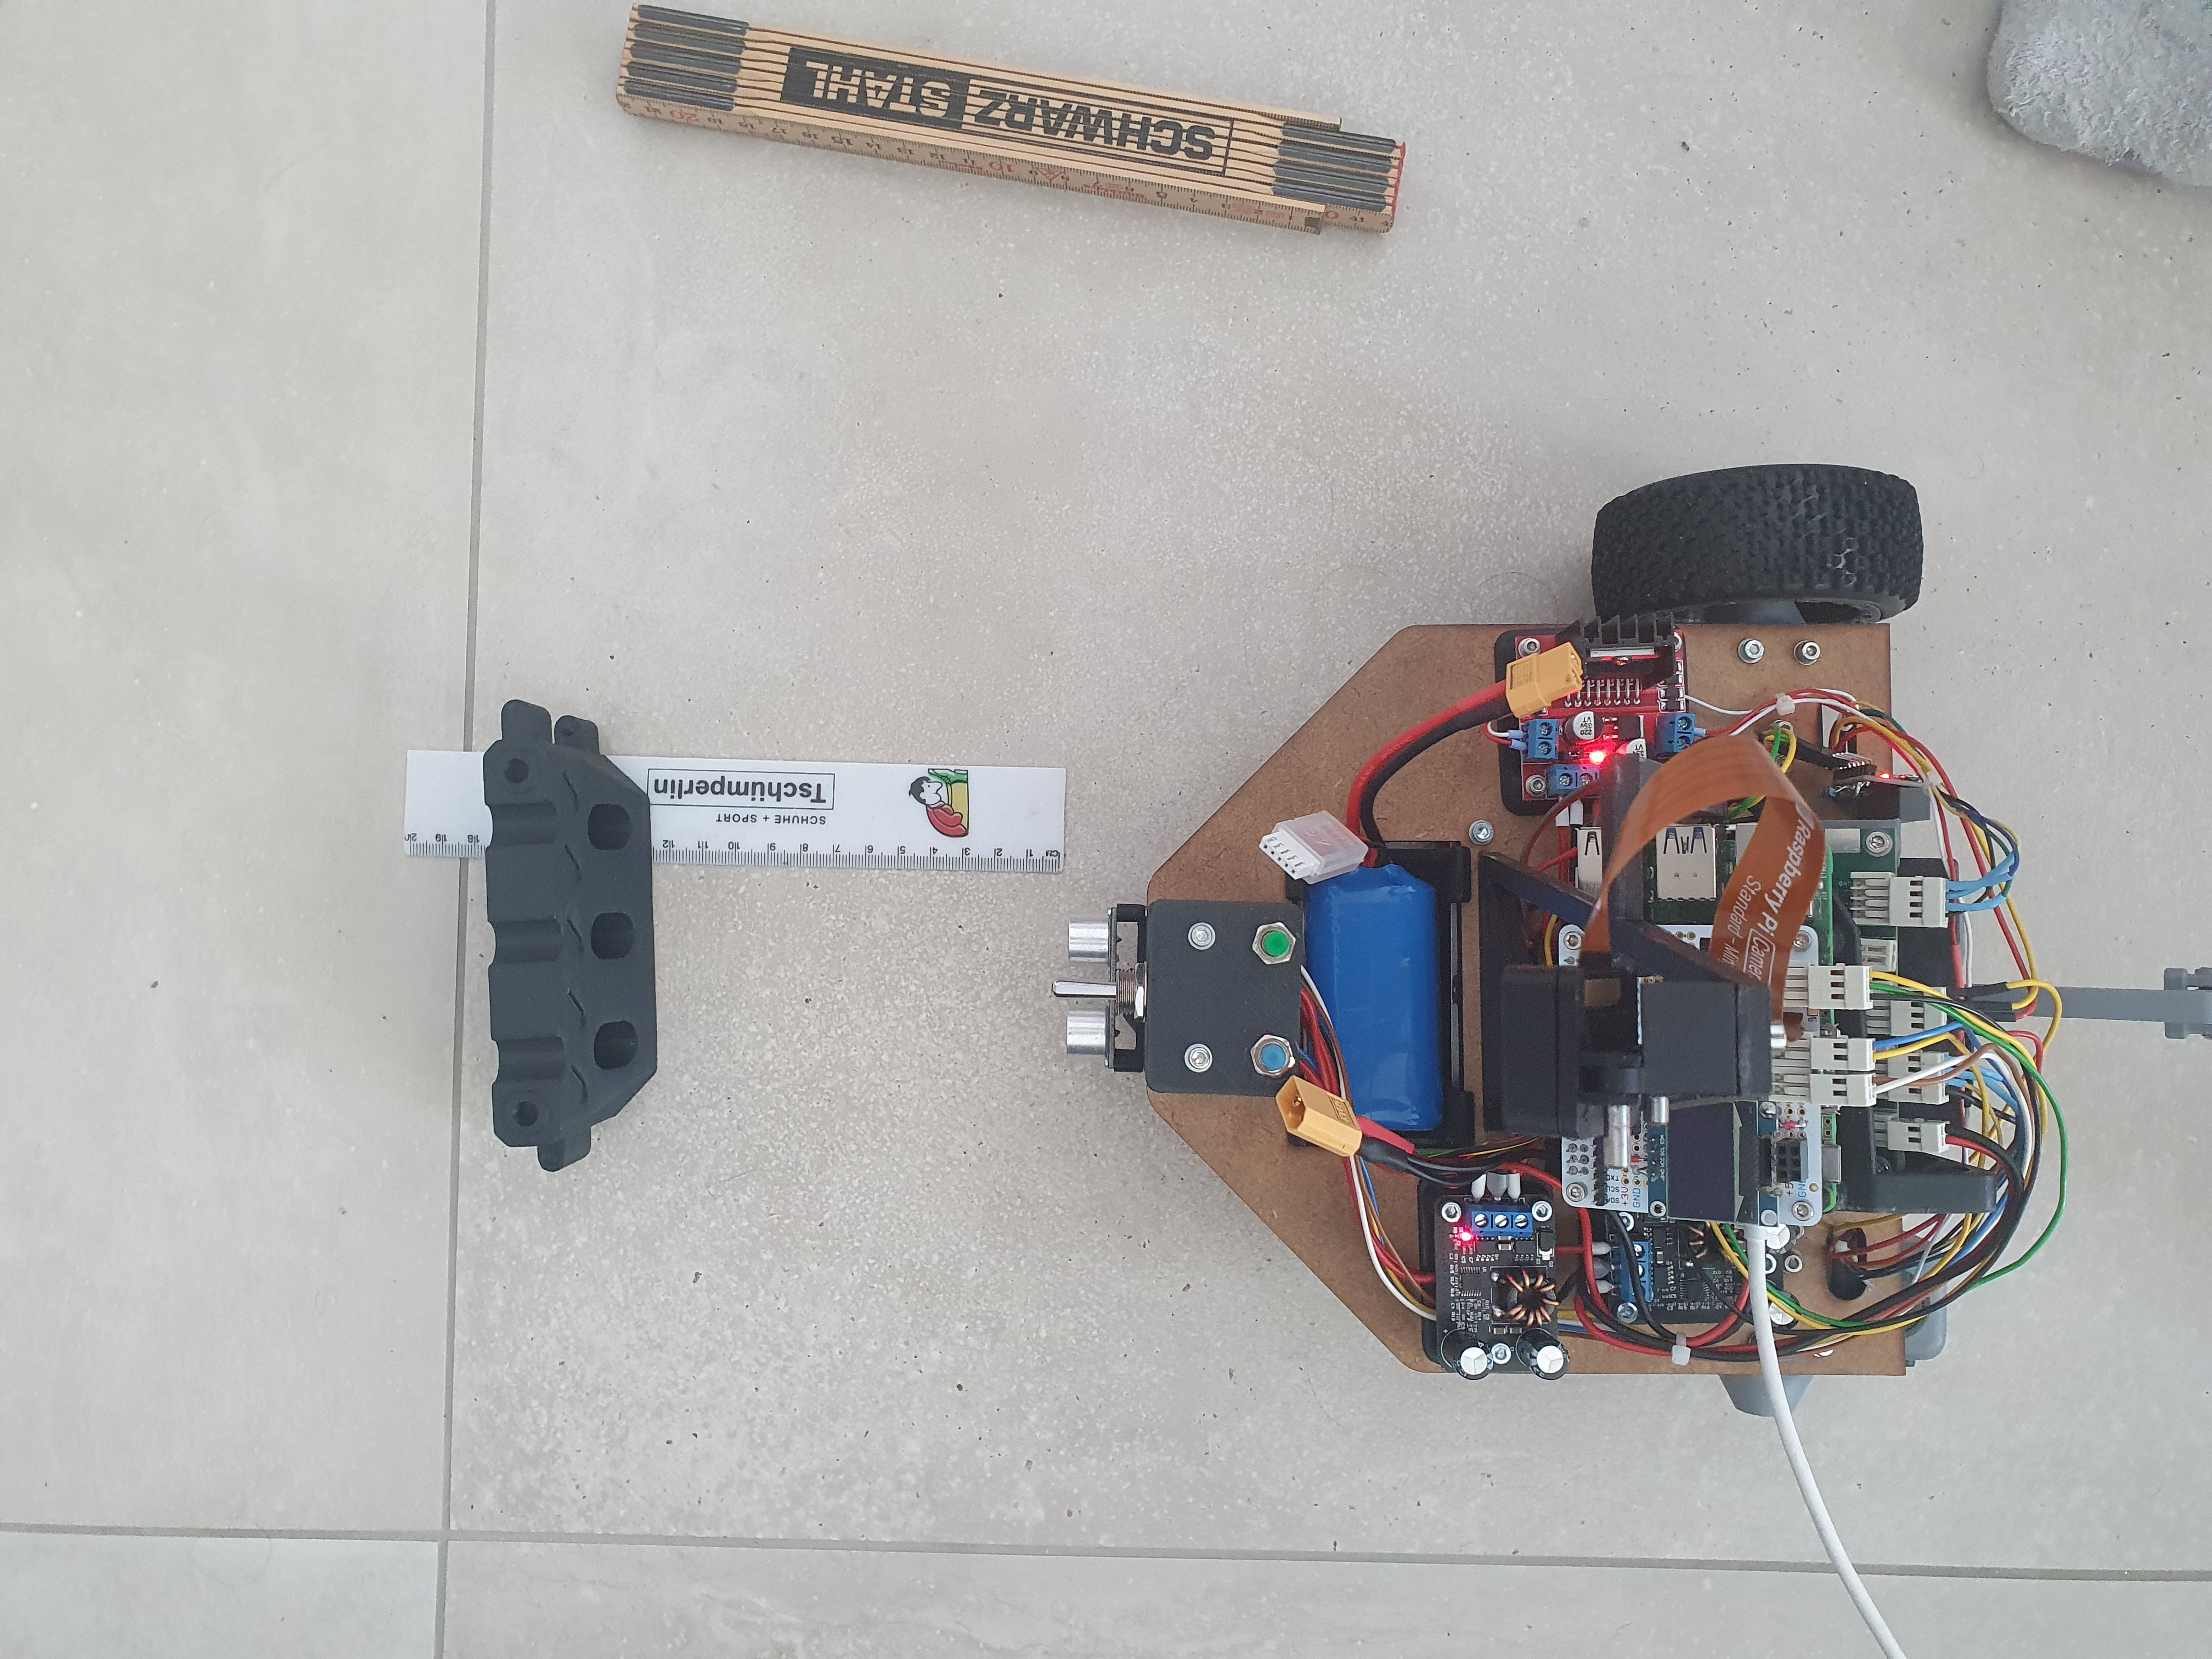
\includegraphics[width=0.5\linewidth]{assets/ET/ultraschall/ultraschall-test.jpg}
    \caption{Ultraschall Testaufbau}
    \label{fig:ultraschall-tests}
\end{figure}

\subsubsection{Kamerahalterung}
\label{Kamera Halter}

Der Winkel und die Höhe der Kamera wurden in \acrshort{pren1} an dem Testaufbau in Abbildung \ref{fig:Testaufbau zum Festlegen des Kamerawinkels} getestet. Am Testaufbau konnte der Winkel zwischen der Kamera und der Vertikalen mit Hilfe einer Schraube verstellt werden. Der Winkel wurde so gewählt, dass er für die Bildverarbeitung ideal ist. 

\begin{figure}[H]
\centering
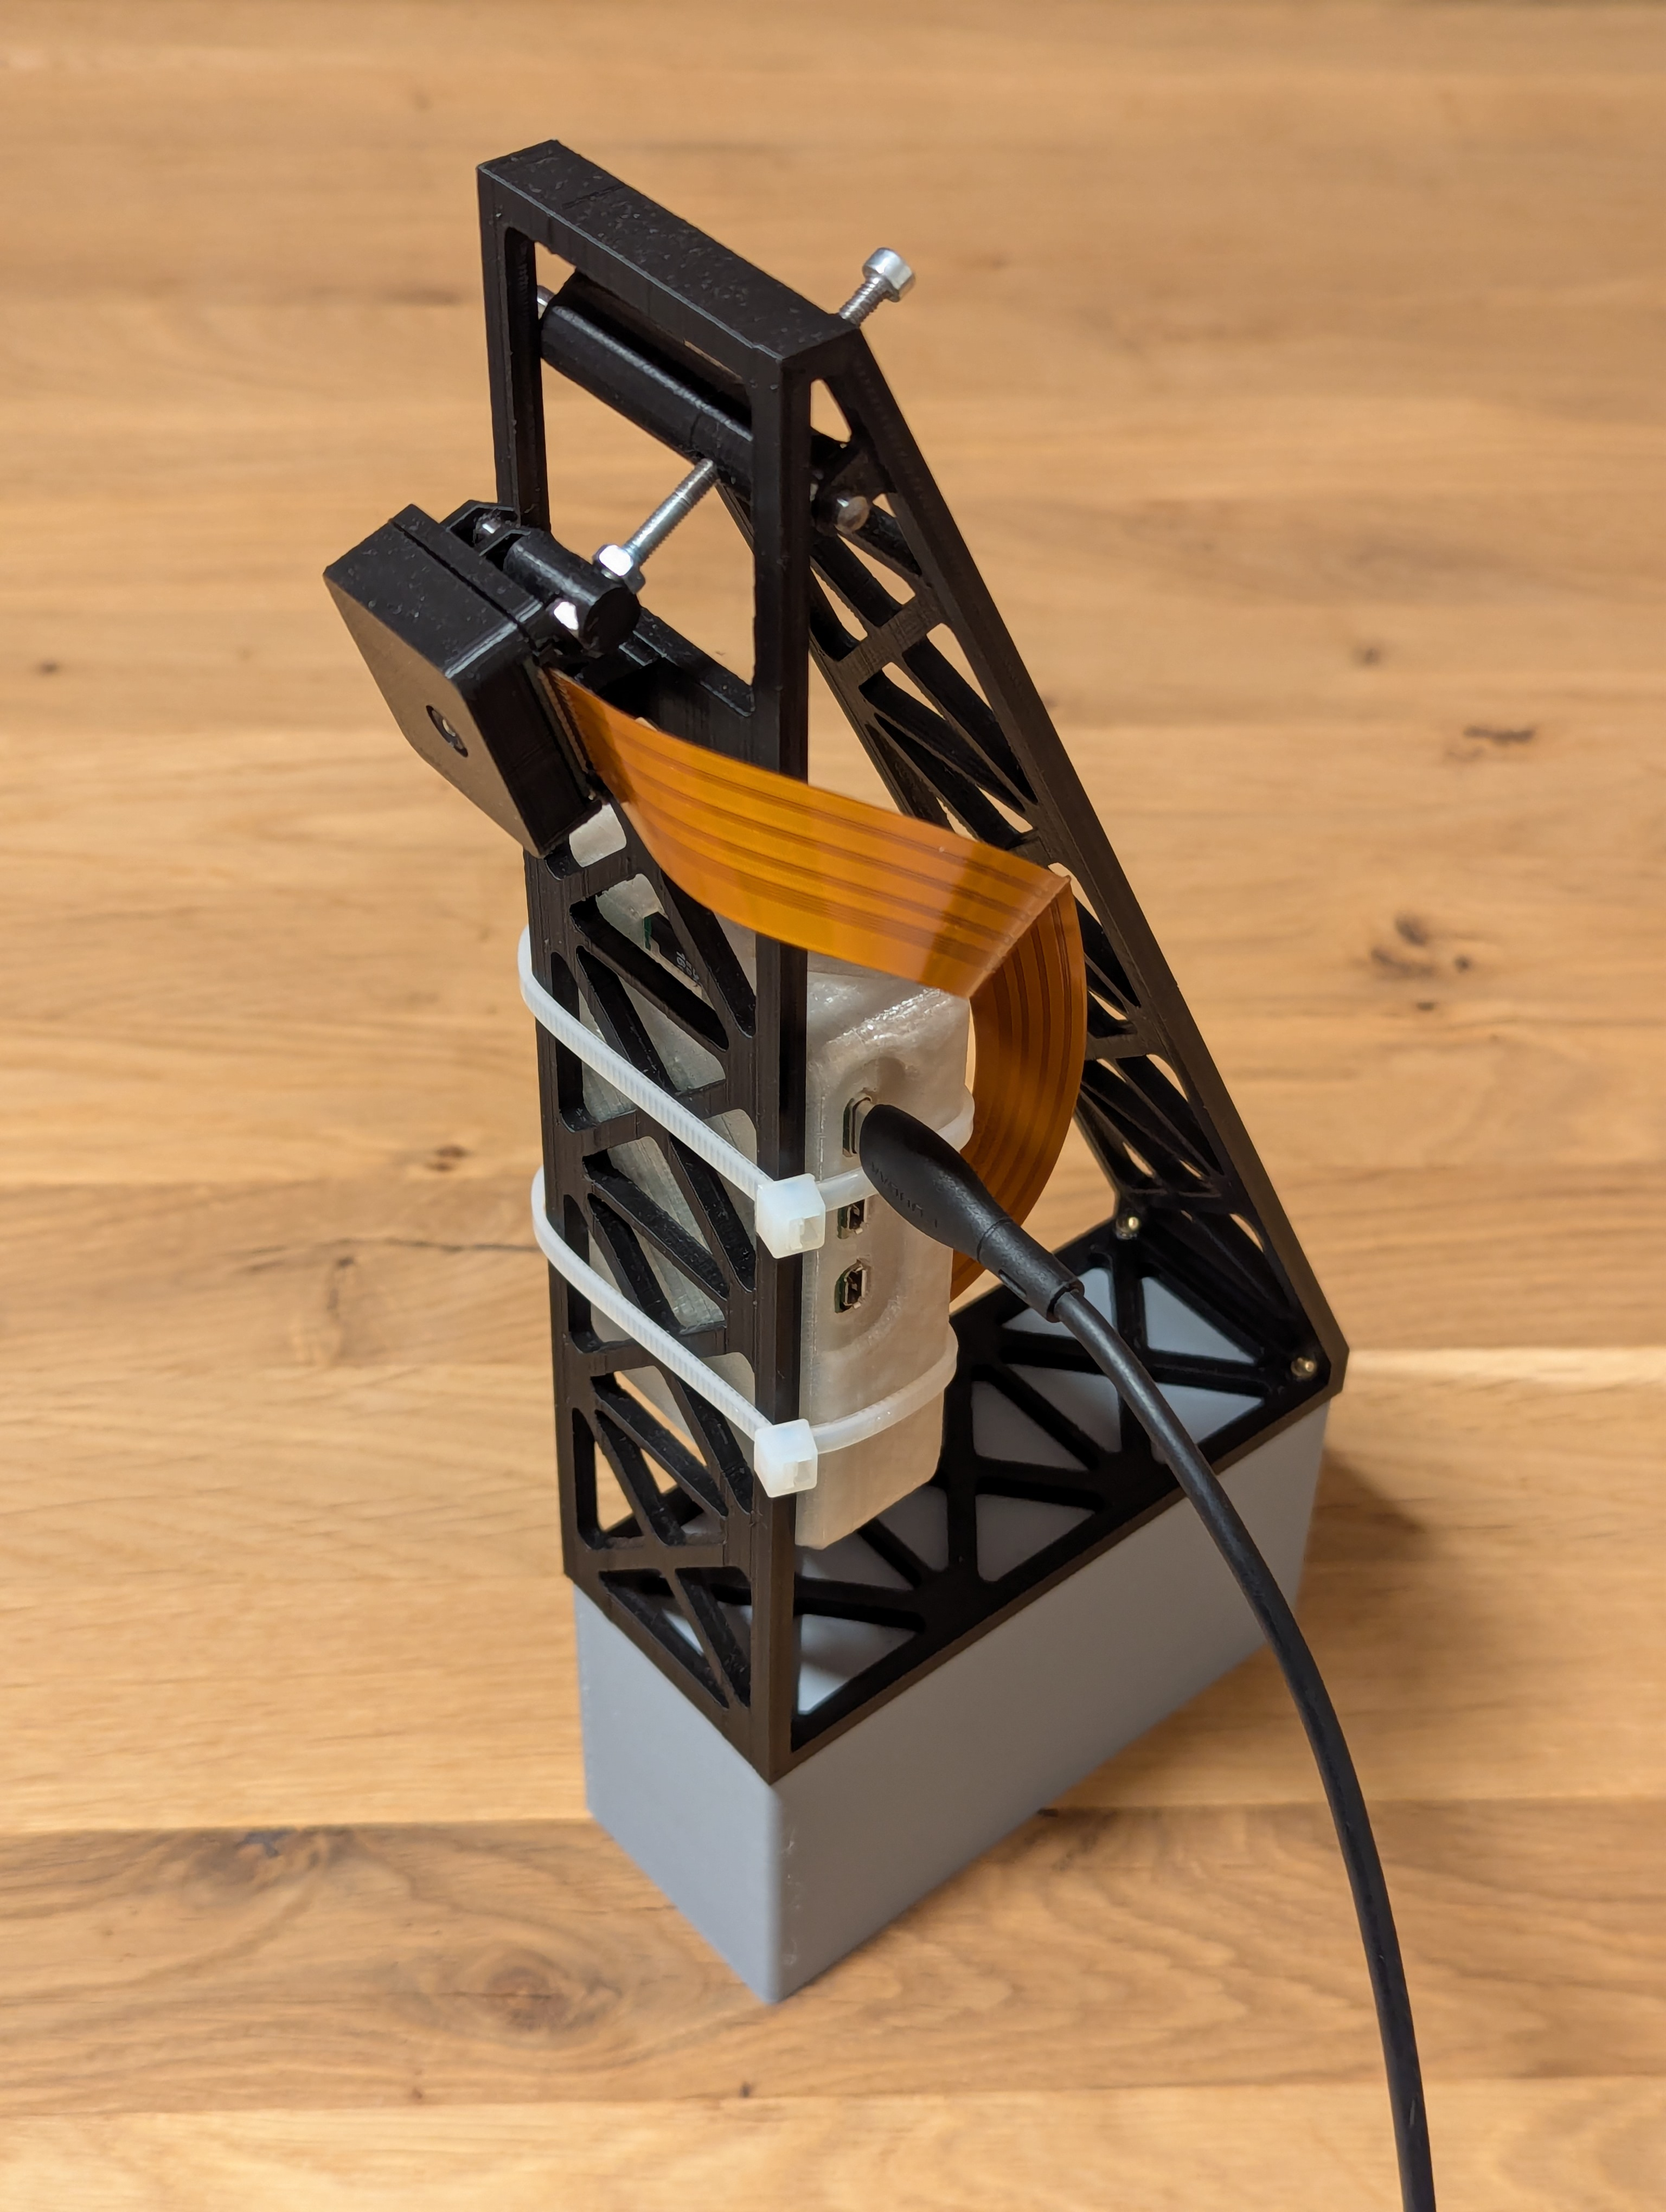
\includegraphics[width=5cm]{assets/MT/camer_tower_2.png}
\caption{Testaufbau zum Festlegen des Kamerawinkels}
\label{fig:Testaufbau zum Festlegen des Kamerawinkels}
\end{figure}


Bei der Konstruktion der Kamerabefestigung wird darauf geachtet, dass der Winkel wie im Testaufbau gemessen 23\textdegree\ beträgt. Ebenfalls wichtig ist, dass die Linsenhöhe 242mm über dem Boden beträgt. Dies wurde in \acrshort{pren1} bereits so definiert, da mit diesen Massen, eine Pylone in zwei Metern Entfernung immer noch komplett sichrbar ist. Der Kameraturm auf dem Roboter ist gezeigt auf Abbildungen \ref{fig:Skizze der Funktionsmasse für die Kamerabefestigung} und \ref{fig:kameraturm-robi}.


\begin{figure}[H]
\centering
\begin{minipage}[b]{0.58\textwidth}
\centering
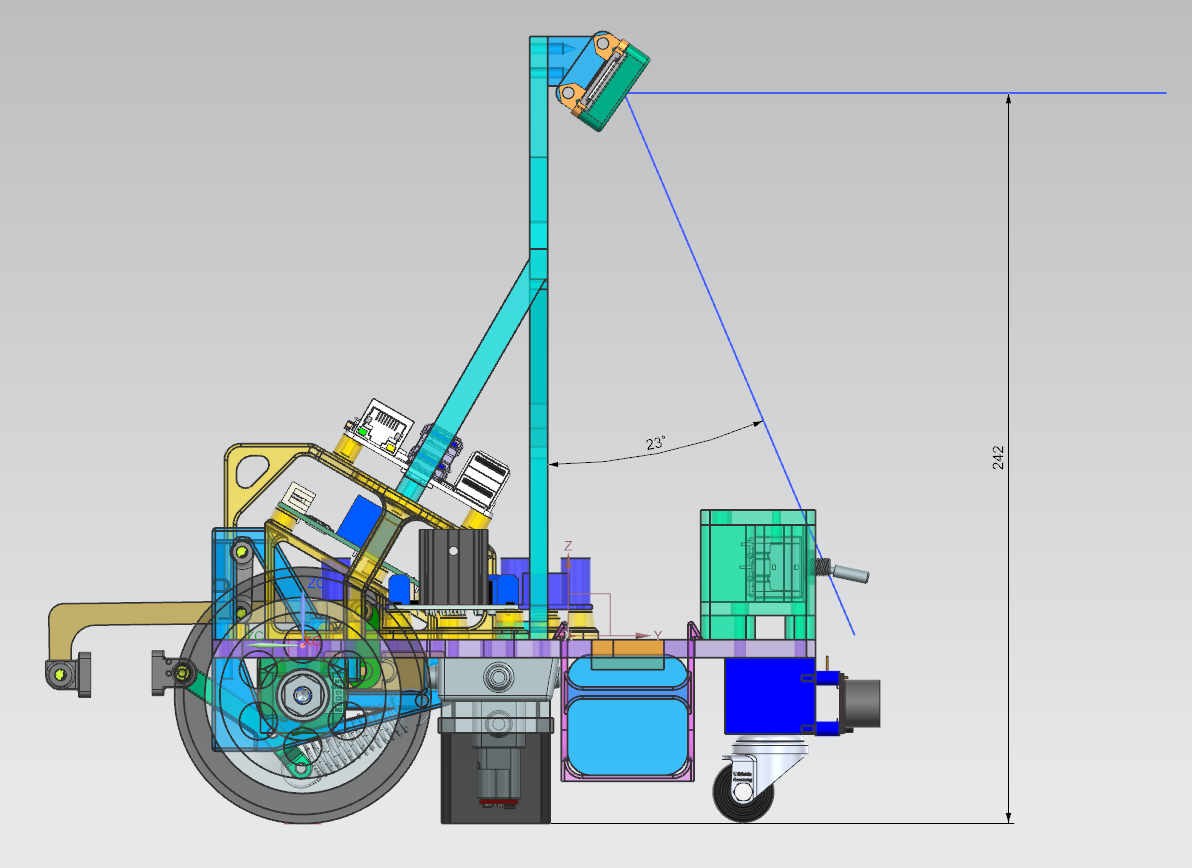
\includegraphics[width= \textwidth ]{assets/MT/Sichtfeld_Roboter.png}
\caption{Skizze der Funktionsmasse für die Kamerabefestigung}
\label{fig:Skizze der Funktionsmasse für die Kamerabefestigung}

\end{minipage}
\hfill
\begin{minipage}[b]{0.41\textwidth}
  \centering
  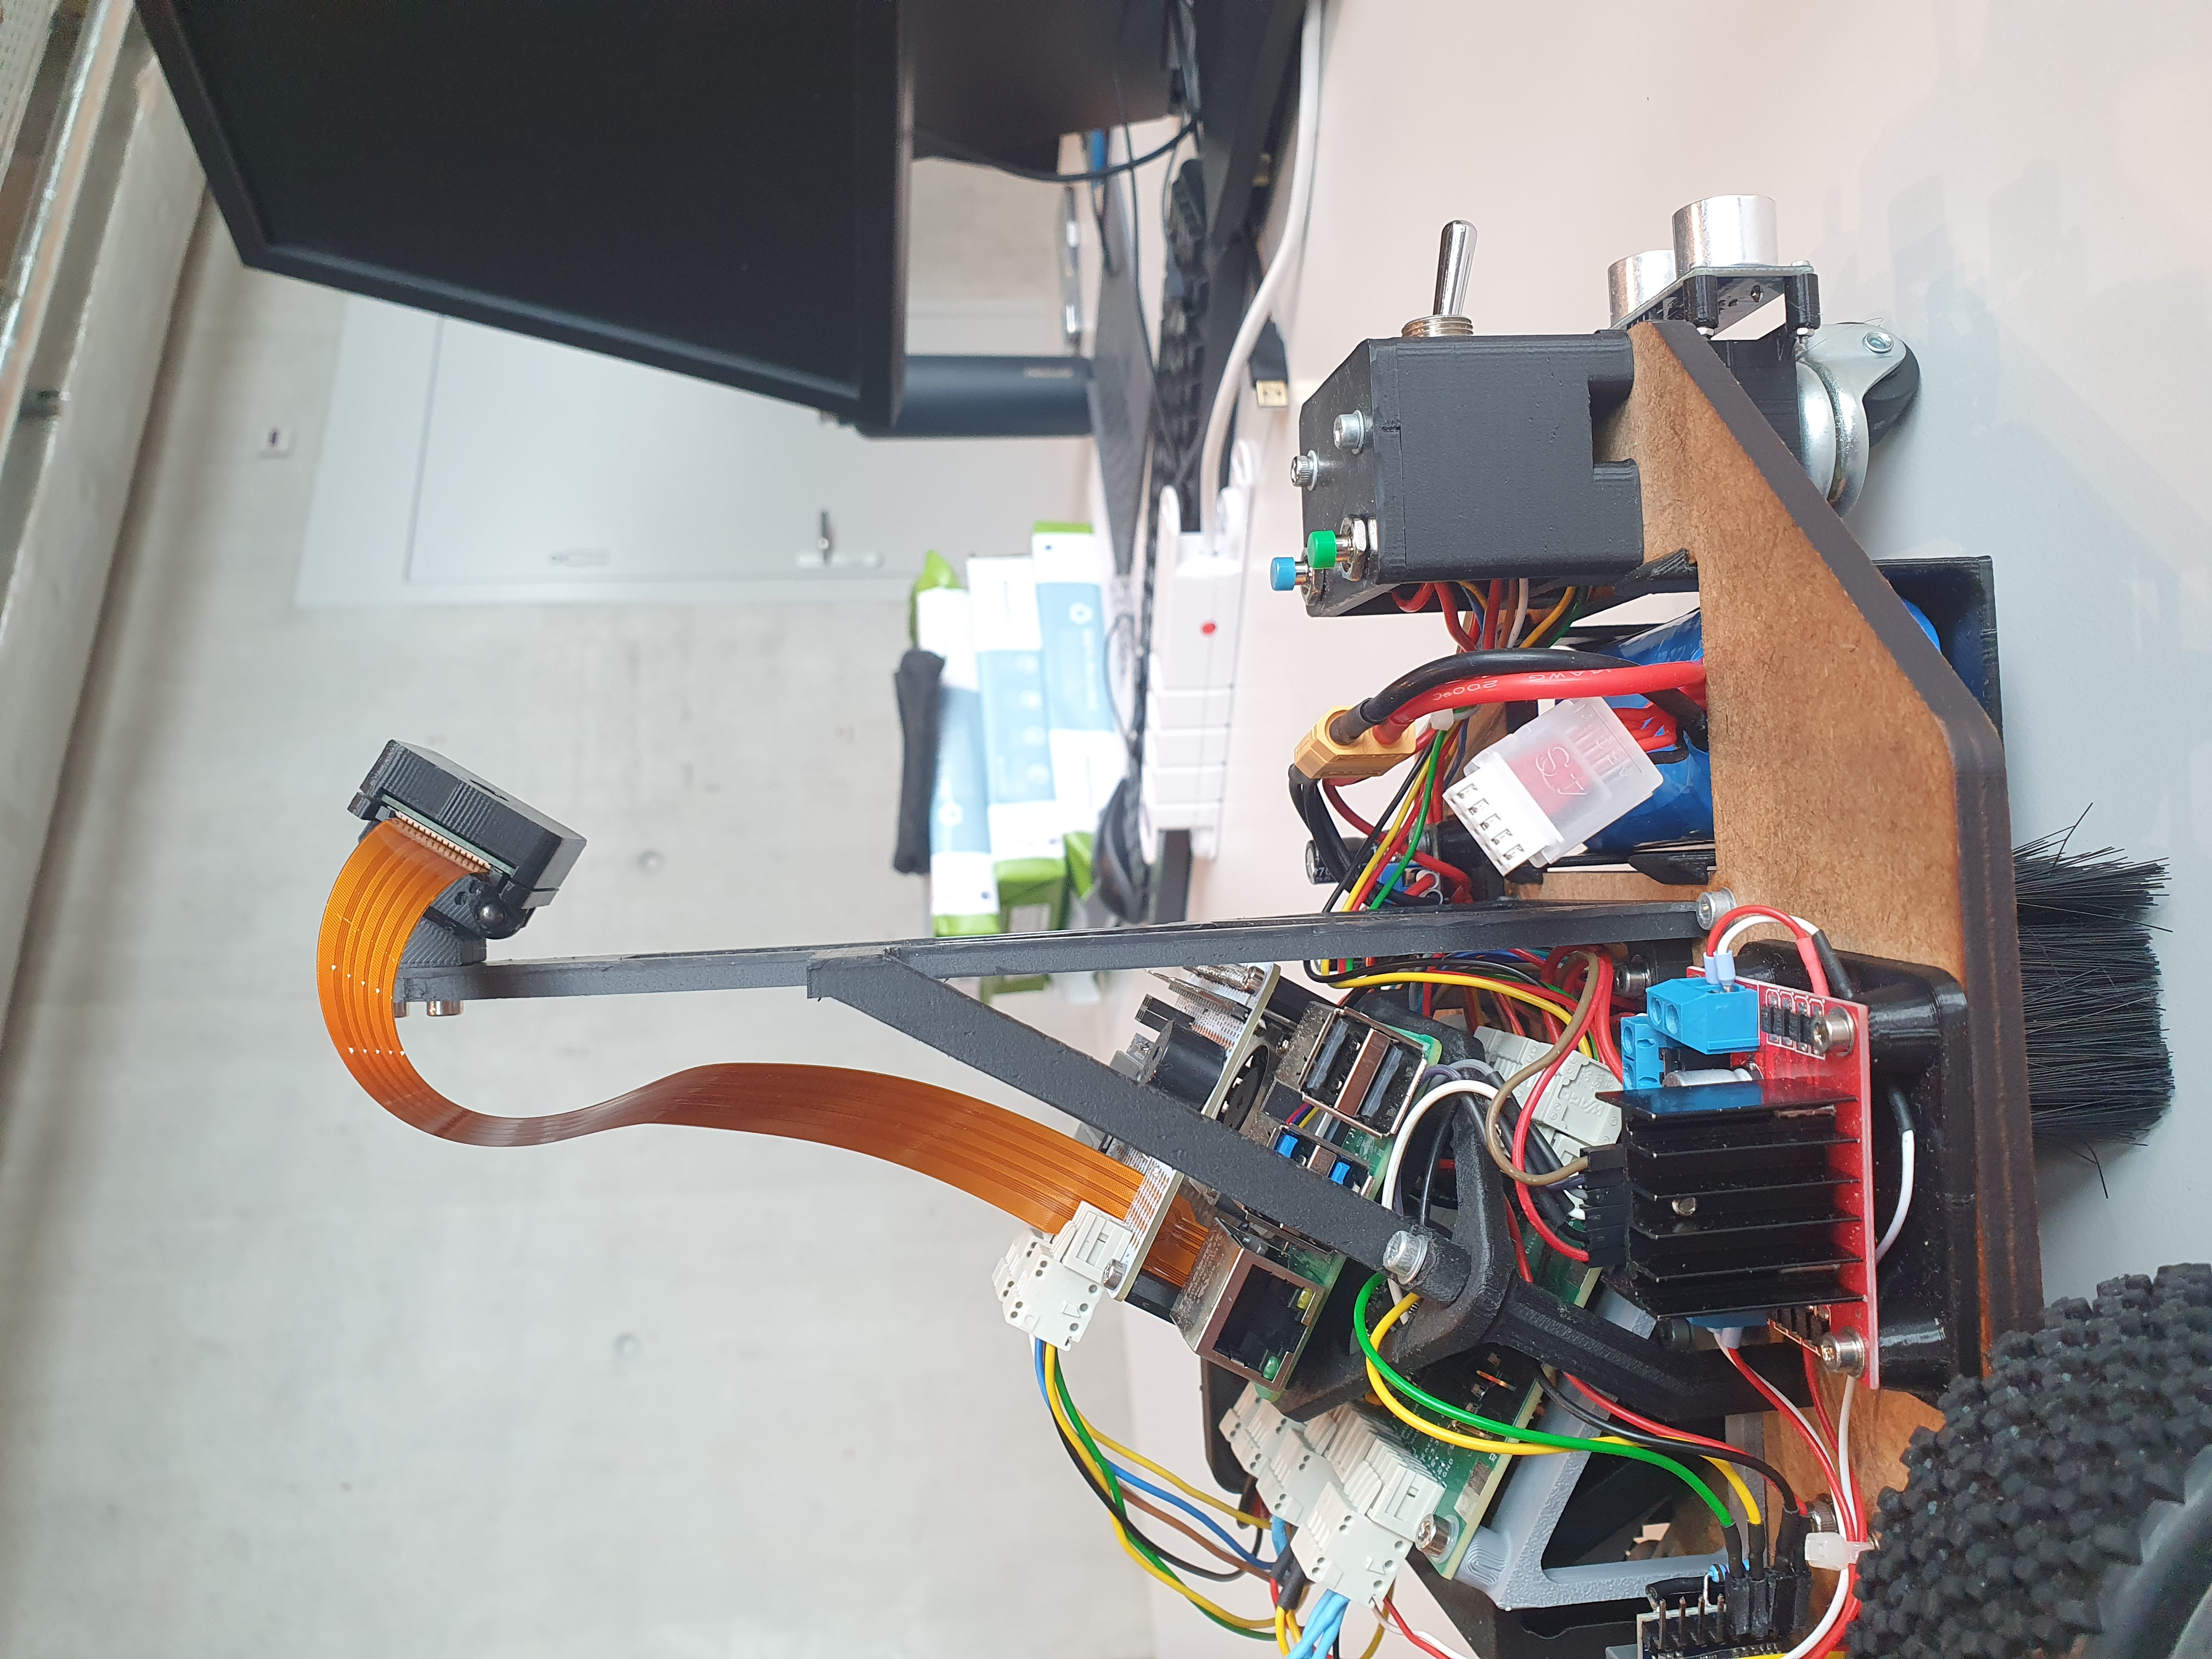
\includegraphics[width=\textwidth, angle=-90]{assets/MT/kamerahalterung.jpg}
  \caption{Kamerahalterung am Roboter angebracht}
  \label{fig:kameraturm-robi}
\end{minipage}
\end{figure}

%%%%%%%%%%%%%%%%%Epic 1%%%%%%%%%%%%%%%%%%%%%%%%%%%%%%%%%%%%%%%%%%%%%%%%%%%%%%%
\subsection{Fortbewegung mit geregelter Geschwindigkeit}

\subsubsection{Print Circuit Board Design}
\label{pcb}

Um eine zuverlässige Kontaktierung der einzelnen Komponenten sicherzustellen, wird im Rahmen von \acrshort{pren2} ein Verbindungs-PCB, ersichtlich auf Abbildung \ref{fig: Verteiler PCB}, entwickelt. Dieses \acrshort{pcb} übernimmt das Management der
Spannungsversorgung für den Raspberry Pi und den \gls{tinyk22}. Zudem werden sämtliche Signale,
die vom \gls{tinyk22} erfasst und verarbeitet werden sollen, entsprechend verbunden.

\begin{figure}[H]
\centering
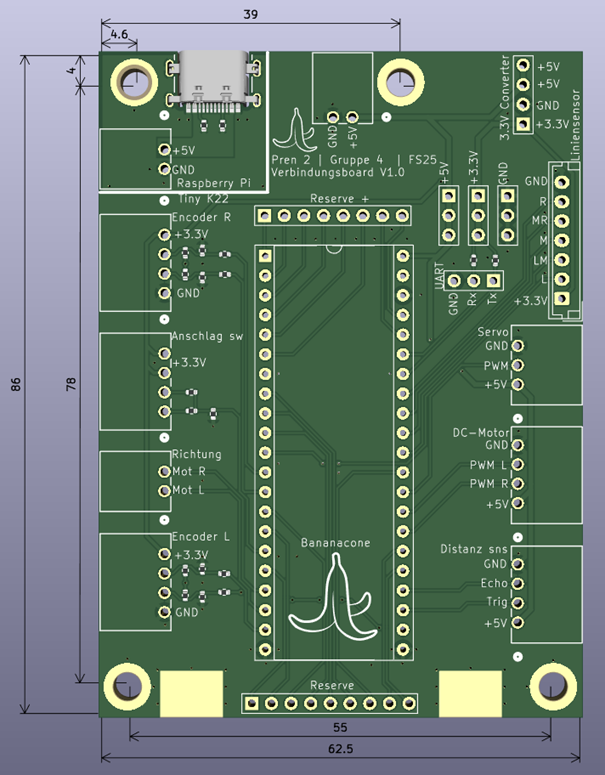
\includegraphics[width=5cm, height=6cm]{assets/ET/PCB/VerteilerPCB_unbestueckt.png}
\caption{Verteiler PCB}
\label{fig: Verteiler PCB}
\end{figure}

Von dem PCB werden fünf Exemplare bestellt. Ebenso sind von dem \gls{tinyk22} mehrere Exemplare vorhanden. Auch von den Motoren gibt es ein zweites Exemplar. Somit ist das Risiko 19 der kaputten Elektroteile (siehe Tabelle \ref{table:risks}) nicht mehr relevant.

Das PCB zusammen mit dem \gls{tinyk22} ist auf Abbildung \ref{fig: Verteiler PCBA} gezeigt. 

\begin{figure}[H]
\centering
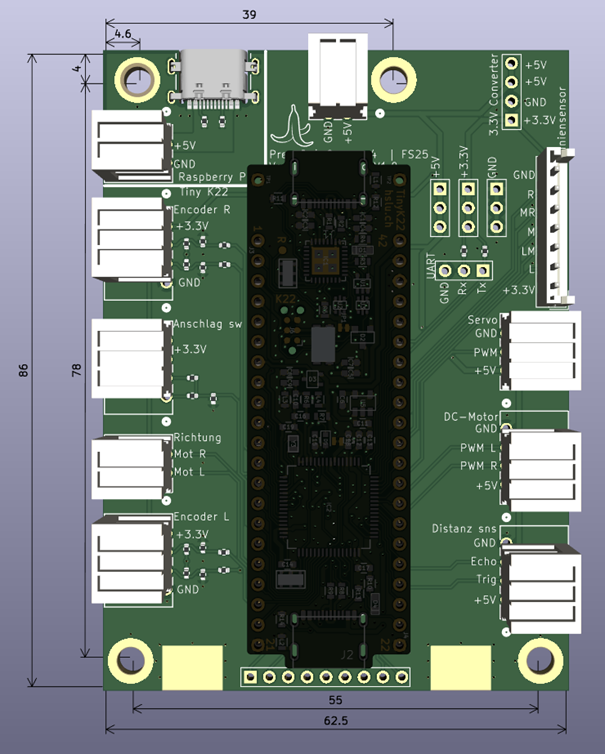
\includegraphics[width=5cm, height=6cm]{assets/ET/PCB/VerteilerPCB_bestueckt.png}
\caption{Verteiler PCBA}
\label{fig: Verteiler PCBA}
\end{figure}


\subsubsection{Pinout und Softwaregrundlagen}

Als Grundlage für die Software diente das Projekt aus dem Modul \textit{Microcontroller Fundamentals}. Dieses enthielt ein solides Gerüst, das im Verlauf des Roboterbaus angepasst wird. Dabei werden verschiedene Codeabschnitte ergänzt, überarbeitet oder entfernt.

Die Initialisierung der Pins erfolgte auf Basis der Belegungen aus Abbildung \ref{fig:Pinout TinyK22} und Abbildung \ref{fig:Pinout Raspy Hat}.

\begin{figure}[H]
\centering
\begin{minipage}[b]{0.45\textwidth}
  \centering
  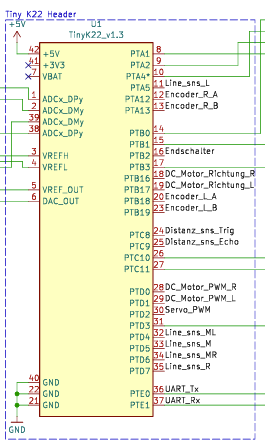
\includegraphics[width=\textwidth]{assets/ET/Software/Tiny_Pinout.png}
  \caption{Pinout Tiny K22}
  \label{fig:Pinout TinyK22}
\end{minipage}
\hspace{0.05\textwidth} % Abstand zwischen den Bildern
\begin{minipage}[b]{0.45\textwidth}
  \centering
  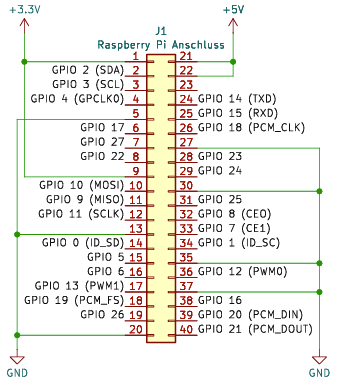
\includegraphics[width=\textwidth]{assets/ET/Software/RaspyHat_Pinout.png}
  \caption{Pinout Raspberry Pi}
  \label{fig:Pinout Raspy Hat}
\end{minipage}
\end{figure}

Im Vergleich zur ursprünglichen Planung in \acrshort{pren1} (siehe Abbildung \ref{fig:Pinout PREN 1}) wird das Pinout in \acrshort{pren2} (siehe Abbildung \ref{fig:Pinout PREN 2}) in mehreren Punkten angepasst.

Drei ursprünglich für die Liniensensoren vorgesehene Pins werden aufgrund der verwendeten Sensorbank entfallen. Der Buzzer sowie der Startknopf werden auf das Raspberry Pi HAT verlagert. Zudem wird die Richtungsauswahl von zwei auf vier Pins erweitert, um eine differenziertere Steuerung zu ermöglichen. Und eine zusätzliche $I^2C$-Schnittstelle wurde implementiert, um weitere Sensoren anbinden zu können. 


\begin{figure}[H]
\centering
\begin{minipage}[b]{0.45\textwidth}
  \centering
  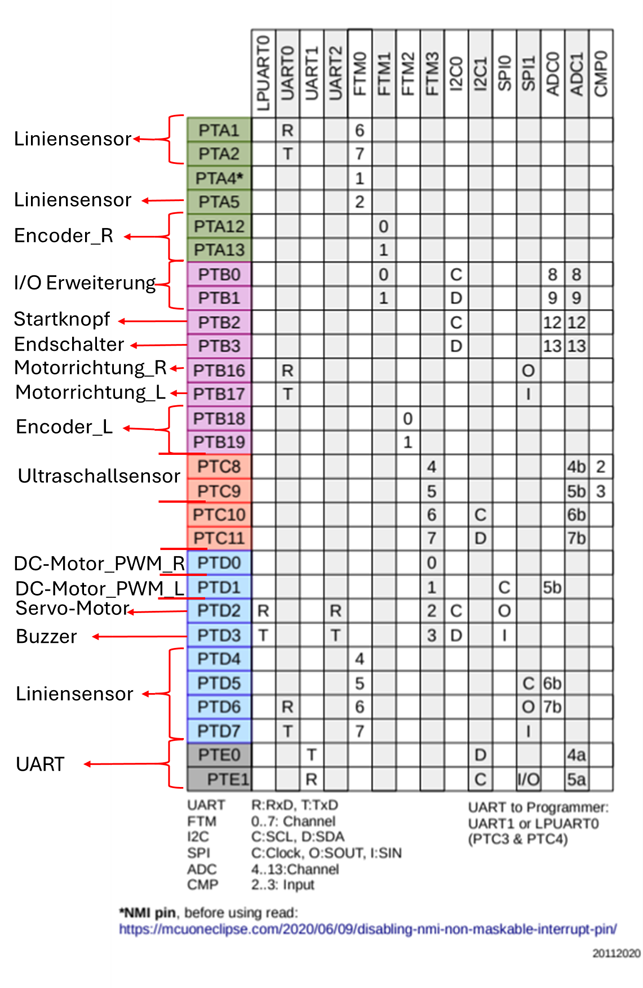
\includegraphics[width=\textwidth]{assets/ET/PINOUT/Pinout_PREN1.png}
  \caption{Pinout PREN 1}
  \label{fig:Pinout PREN 1}
\end{minipage}
\hspace{0.05\textwidth} % Abstand zwischen den Bildern
\begin{minipage}[b]{0.45\textwidth}
  \centering
  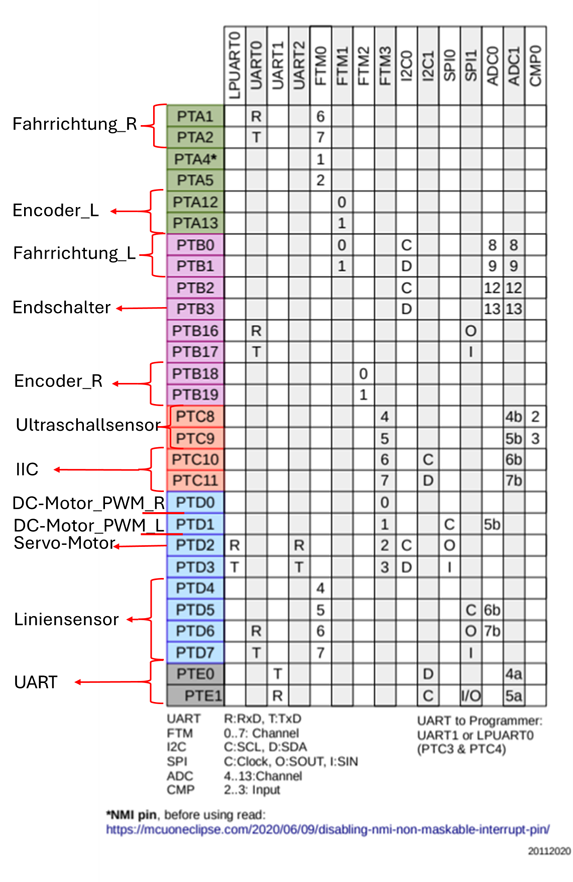
\includegraphics[width=\textwidth]{assets/ET/PINOUT/Pinout_PREN2.png}
  \caption{Pinout PREN 2}
  \label{fig:Pinout PREN 2}
\end{minipage}
\end{figure}





\subsubsection{Spannungsversorgung und Leistungsberechnung}


In der Tabelle \ref{tab:spannungsversorgung} werden alle Verbraucher mit ihrer Betriebsspannung aufgezeigt, wie auch die maximalen Stromaufnahme. Anhand dieser Daten kann die Wahl eines geeigneten Akkus getroffen werden.

Die Spannungsversorgung kann mittels eines Not-Aus Schalters von den Verbrauchern getrennt werden. Das Raspberry Pi 5 wird dabei als einziger Verbraucher nicht von der Spannung getrennt (siehe Abbildung \ref{fig: Verdrahtung Hauptschalter}). Damit wird die Möglichkeit von Datenkorruption auf der SD-Karte verringert.

Wird von jedem Verbraucher die Leistung berechnet, ist dies eine maximale Gesamtleistung von 101W (siehe Berechnung \ref{eq:Energieverbrauch}). Der vorgesehene Akku, liefert eine Spannung von 14.8V und eine Kapazität von 3000mAh. Unter maximaler Leistung könnte der Roboter für ca. 25 Minuten betrieben werden. .

\begin{equation}
    t = \frac{E}{P} = \frac{U \cdot Q}{P} = \frac{14{,}8\,\text{V} \cdot 10800\,\text{As}}{105\,\text{W}} \approx 1{'}520\,\text{s} = 25\,\text{Minuten} 
    \label{eq:Energieverbrauch}
\end{equation}


\newpage

\begin{table}[H]
\centering
\renewcommand{\arraystretch}{1.3}
\begin{tabularx}{\textwidth}{|l|c|c|X|}
\hline
\textbf{Verbraucher} & \textbf{Spannung} & \textbf{Strom (geschätzt)} & \textbf{Bemerkung} \\
\hline
2x DC-Motor & 12V & 6A gesamt & Ansteuerung über Motortreiber \\
\hline
Motortreiber & 5V &  100mA & Logikversorgung \\
\hline
2x Encoder & 3.3V &  150mA gesamt &- \\
\hline
Servomotor & 5V &  500mA & PWM-gesteuert, kurzzeitig hohe Last \\
\hline
Liniensensor & 5V &  150mA & IR-LED's und Sensoren \\
\hline
Ultraschall & 5V &  200mA &- \\
\hline
Raspberry Pi 5 & 5V & 3-5A & über USB-C \\
\hline
Tiny K22 & 5V & 500mA & - \\
\hline
\end{tabularx}
\caption{Übersicht der Spannungsversorgung des Roboters}
\label{tab:spannungsversorgung}
\end{table}





\subsubsection{Motoren ansteuern und auslesen}
\label{motoren-encoder}

Um die Motoren richtig anzusteuern, werden die Ticks der Encoder pro Radumdrehung in der MCCAR Library in dem Quad Modul definiert. Danach wird mithilfe eines Lineals geprüft, ob der Roboter sich die Distanz vorbewegt, wie der Encoder dies vorgibt. Da dies erfolgreich war, kann das Drive Modul der Library verwendet werden. Damit sich die Motoren so schnell drehen, wie in den jeweiligen Ziel-Variablen vorgegeben. Mit der konfigurierten Library soll der Roboter in der Lage sein, eine bestimmte Distanz akkurat zurückzulegen. Wie in \acrshort{pren1} geplant, werden Motoren mit Encodern gewählt, um die Fahrdistanz auslesen zu können.

Nachdem die erste Ausführung der Software für die Motoren mit den beiden Encodern vorhanden ist, wird der implementierte Code mithilfe eines provisorischen Aufbaus getestet. Unter einem provisorischen Aufbau versteht sich die Verwendung eines Breadboards mit dem \gls{tinyk22} und einem Speisegerät, anstelle einer richtigen Verbindung mit einem \acrshort{pcb}. Dies ist auf Abbildung \ref{fig: Motorentest} ersichtlich.

\begin{figure}[H]
\centering
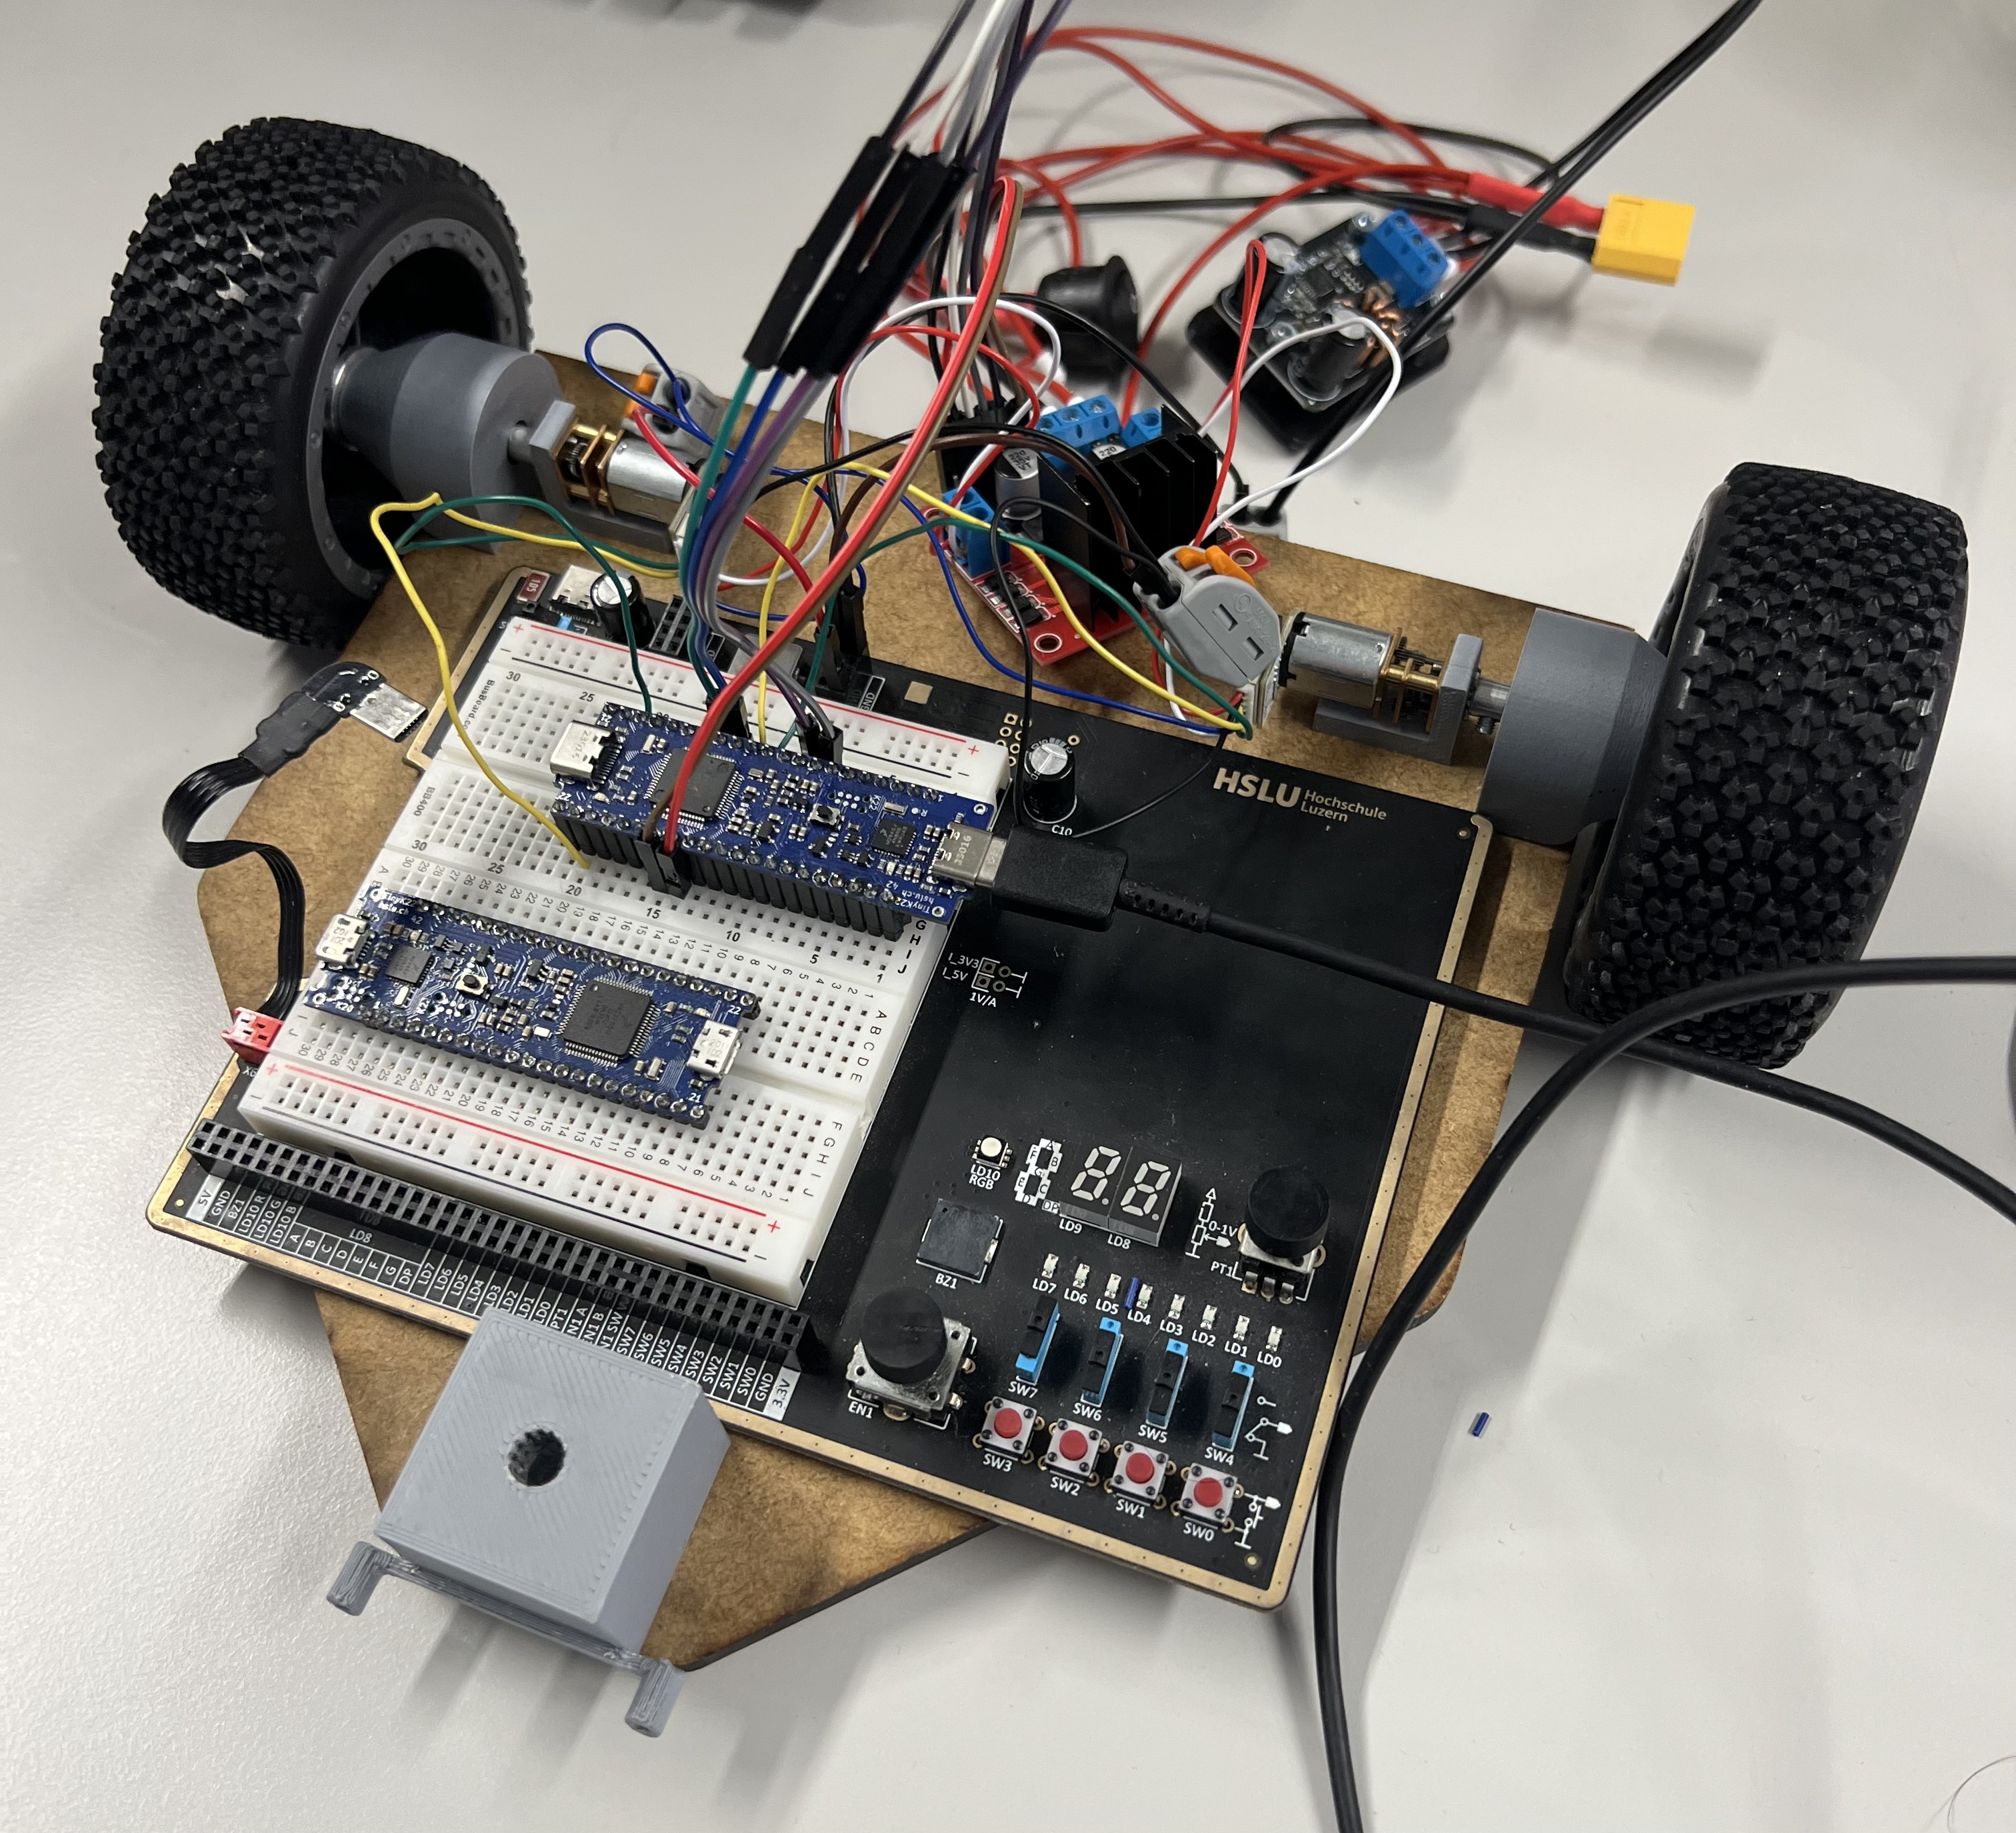
\includegraphics[width=10cm, height=8cm]{assets/ET/Motoren/Motorentest.jpeg}
\caption{Motorentest}
\label{fig: Motorentest}
\end{figure}

Der zugrunde liegende Fahralgorithmus basiert darauf, die Werte beider Encoder zu mitteln, um die gefahrene Strecke zu ermitteln (siehe Berechnung \ref{eq:gefahren}).

\begin{equation}
    gefahrenMEAN_{cm} = \frac{gefahrenR_{cm} + gefahrenL_{cm}} {2} 
    \label{eq:gefahren}
\end{equation}







%%%%%%%%%%%%%%%%%Epic 2%%%%%%%%%%%%%%%%%%%%%%%%%%%%%%%%%%%%%%%%%%%%%%%%%%%%%%%

\subsection{Auf Linien des Graphes bewegen}
\label{Auf Linien des Graphes bewegen}

\subsubsection{Liniensensor auslesen}
\label{Liniensensor auslesen}

In einem ersten Durchlauf wird ein Code implementiert, um die Funktion mit dem \gls{tinyk22} zu testen. Mittels eines Timers werden die einzelnen Pins in einem genügend grossen Zeitabstand von \acrfull{vcc} auf Input Capture umgeschaltet. Nach dem Umschalten auf Input Capture, sollen sich die Kondensatoren, die sich am Liniensensor befinden, je nach Reflektion des Untergrundes in unterschiedlichen Zeiten laden. Dieses Verhalten konnte im Testprogramm, durch die unterschiedlichen Werte im Timer Register des Input Capture Modus, erfolgreich festgestellt werden.

Auf der Abbildung \ref{fig:liniensensor soll} ist, während des Traversieren auf der Linie, die Sollposition des Liniensensors gezeigt. Im Konzept von \acrshort{pren1} waren jeweils vor und hinter dem Array ein zusätzlicher Sensor vorgesehen. Jedoch kann dies nicht realisiert werden, da es nicht genügend Timer Channels zur Verfügung hat.

 \begin{figure}[H]
\centering
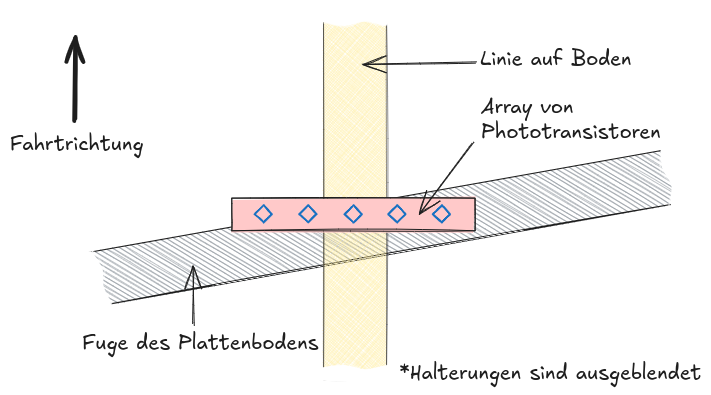
\includegraphics[width=0.5\textwidth ]{assets/ET/Liniensensor/linesensor.png}
\caption{Sollposition Liniensensor während des Fahrens}
\label{fig:liniensensor soll}
\end{figure}


\subsubsection{Linie folgen mit PD-Regelung}
\label{Linie folgen mit PD-Regelung}

Nachdem die Auslesung des Liniensensors erfolgreich getestet wurde, kann die eigentliche Linienregelung implementiert werden, wovon ein Ausschnitt auf Abbildung \ref{fig:Ausschnitt der Implementation der PD-Regelung} ersichtlich ist. Damit möglichst dynamisch und mit möglichst wenig Schwingungen gefahren werden kann, wird ein PD-Regler ausgewählt.

Durch das Ummuxen der Pins von GPIO-Output (High) auf den Input Capture Modus, wird die Ladezeit eines Kondensators gemessen. Diese Zeit (ausgedrückt in Ticks) liefert Informationen darüber, ob sich das Fahrzeug über dem Soll-Fahrweg befindet oder davon abweicht.

Bei jedem Neustart des Roboters, liest eine Kalibrierungsfunktion die Soll-Werte der einzelnen Sensoren ein. Beim Kalibrieren muss der Roboter immer in seiner Soll-Fahrposition stehen.

Die periodisch aufgerufene Reglerfunktion berechnet dann aus dem Soll-Wert und dem aktuellen Sensorwert (Ist-Wert) die Abweichung. Diese Fehler werden zu einem Gesamtfehler mit einer Gewichtung der Sensoren von aussen nach innen zunehmend berechnet. Dieser Gesamtfehler wird dann mit dem P- und D-Anteil zu einem Korrekturwert weiter verrechnet. Der Proportionalanteil (P) sorgt dafür, dass das Fahrzeug bei einem grösseren Fehler stärker korrigiert, während der Differentialanteil (D) auf schnelle Änderungen des Fehlers reagiert und so Schwingungen dämpft. Der Korrekturwert wird dann genutzt um die beiden \acrfull{pwm} Signale der Motoren zu senken oder erhöhen, je nach Abweichung zur Linie.

Während der Fahrt werden die Sensor-Pins periodisch zwischen GPIO High und Input Capture umgeschaltet, um kontinuierlich neue Messwerte zu erhalten. Die erfassten Ticks werden in einer PD-Regelung weiter verarbeitet, welche die Abweichung zur Soll-Position (Linie) berechnet und entsprechend die Motoren nachsteuert. Diese Regelung ergänzt die Wegmessung über die Encodersensoren und erhöht die Spurtreue, indem sie sicherstellt, dass das Fahrzeug die Linie nicht verlässt. 

 \begin{figure}[H]
\centering
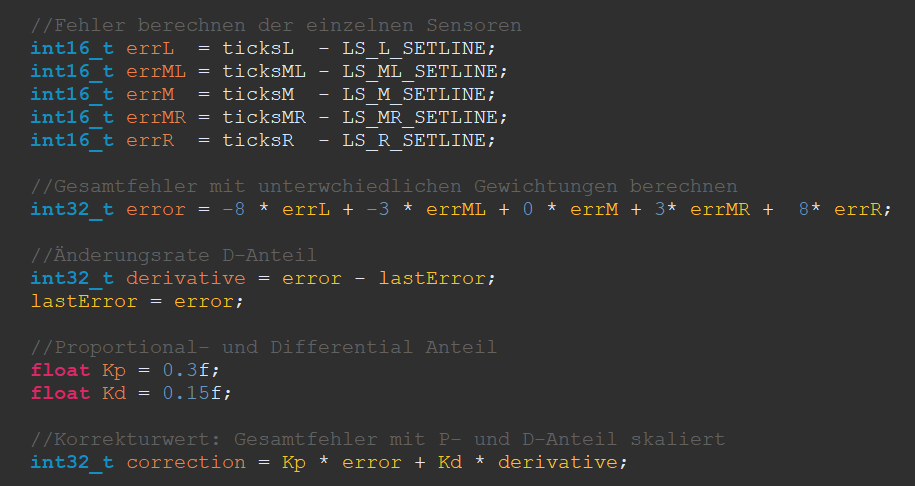
\includegraphics[width= \textwidth ]{assets/ET/PD-Regler/PD-Regler_Code_Pren2.png}
\caption{Ausschnitt der Implementation der PD-Regelung}
\label{fig:Ausschnitt der Implementation der PD-Regelung}
\end{figure}


Der Liniensensor wird am Fahrzeug mit der Abschirmung angebracht (siehe Abbildung \ref{fig:linsen-robi}). Für die Feineinstellung werden die einzelnen Sensorwerte auf dem Originalboden und dem Klebeband ausgemessen, da dies essenziell ist, um die Regelung sauber abzustimmen.

 \begin{figure}[H]
\centering
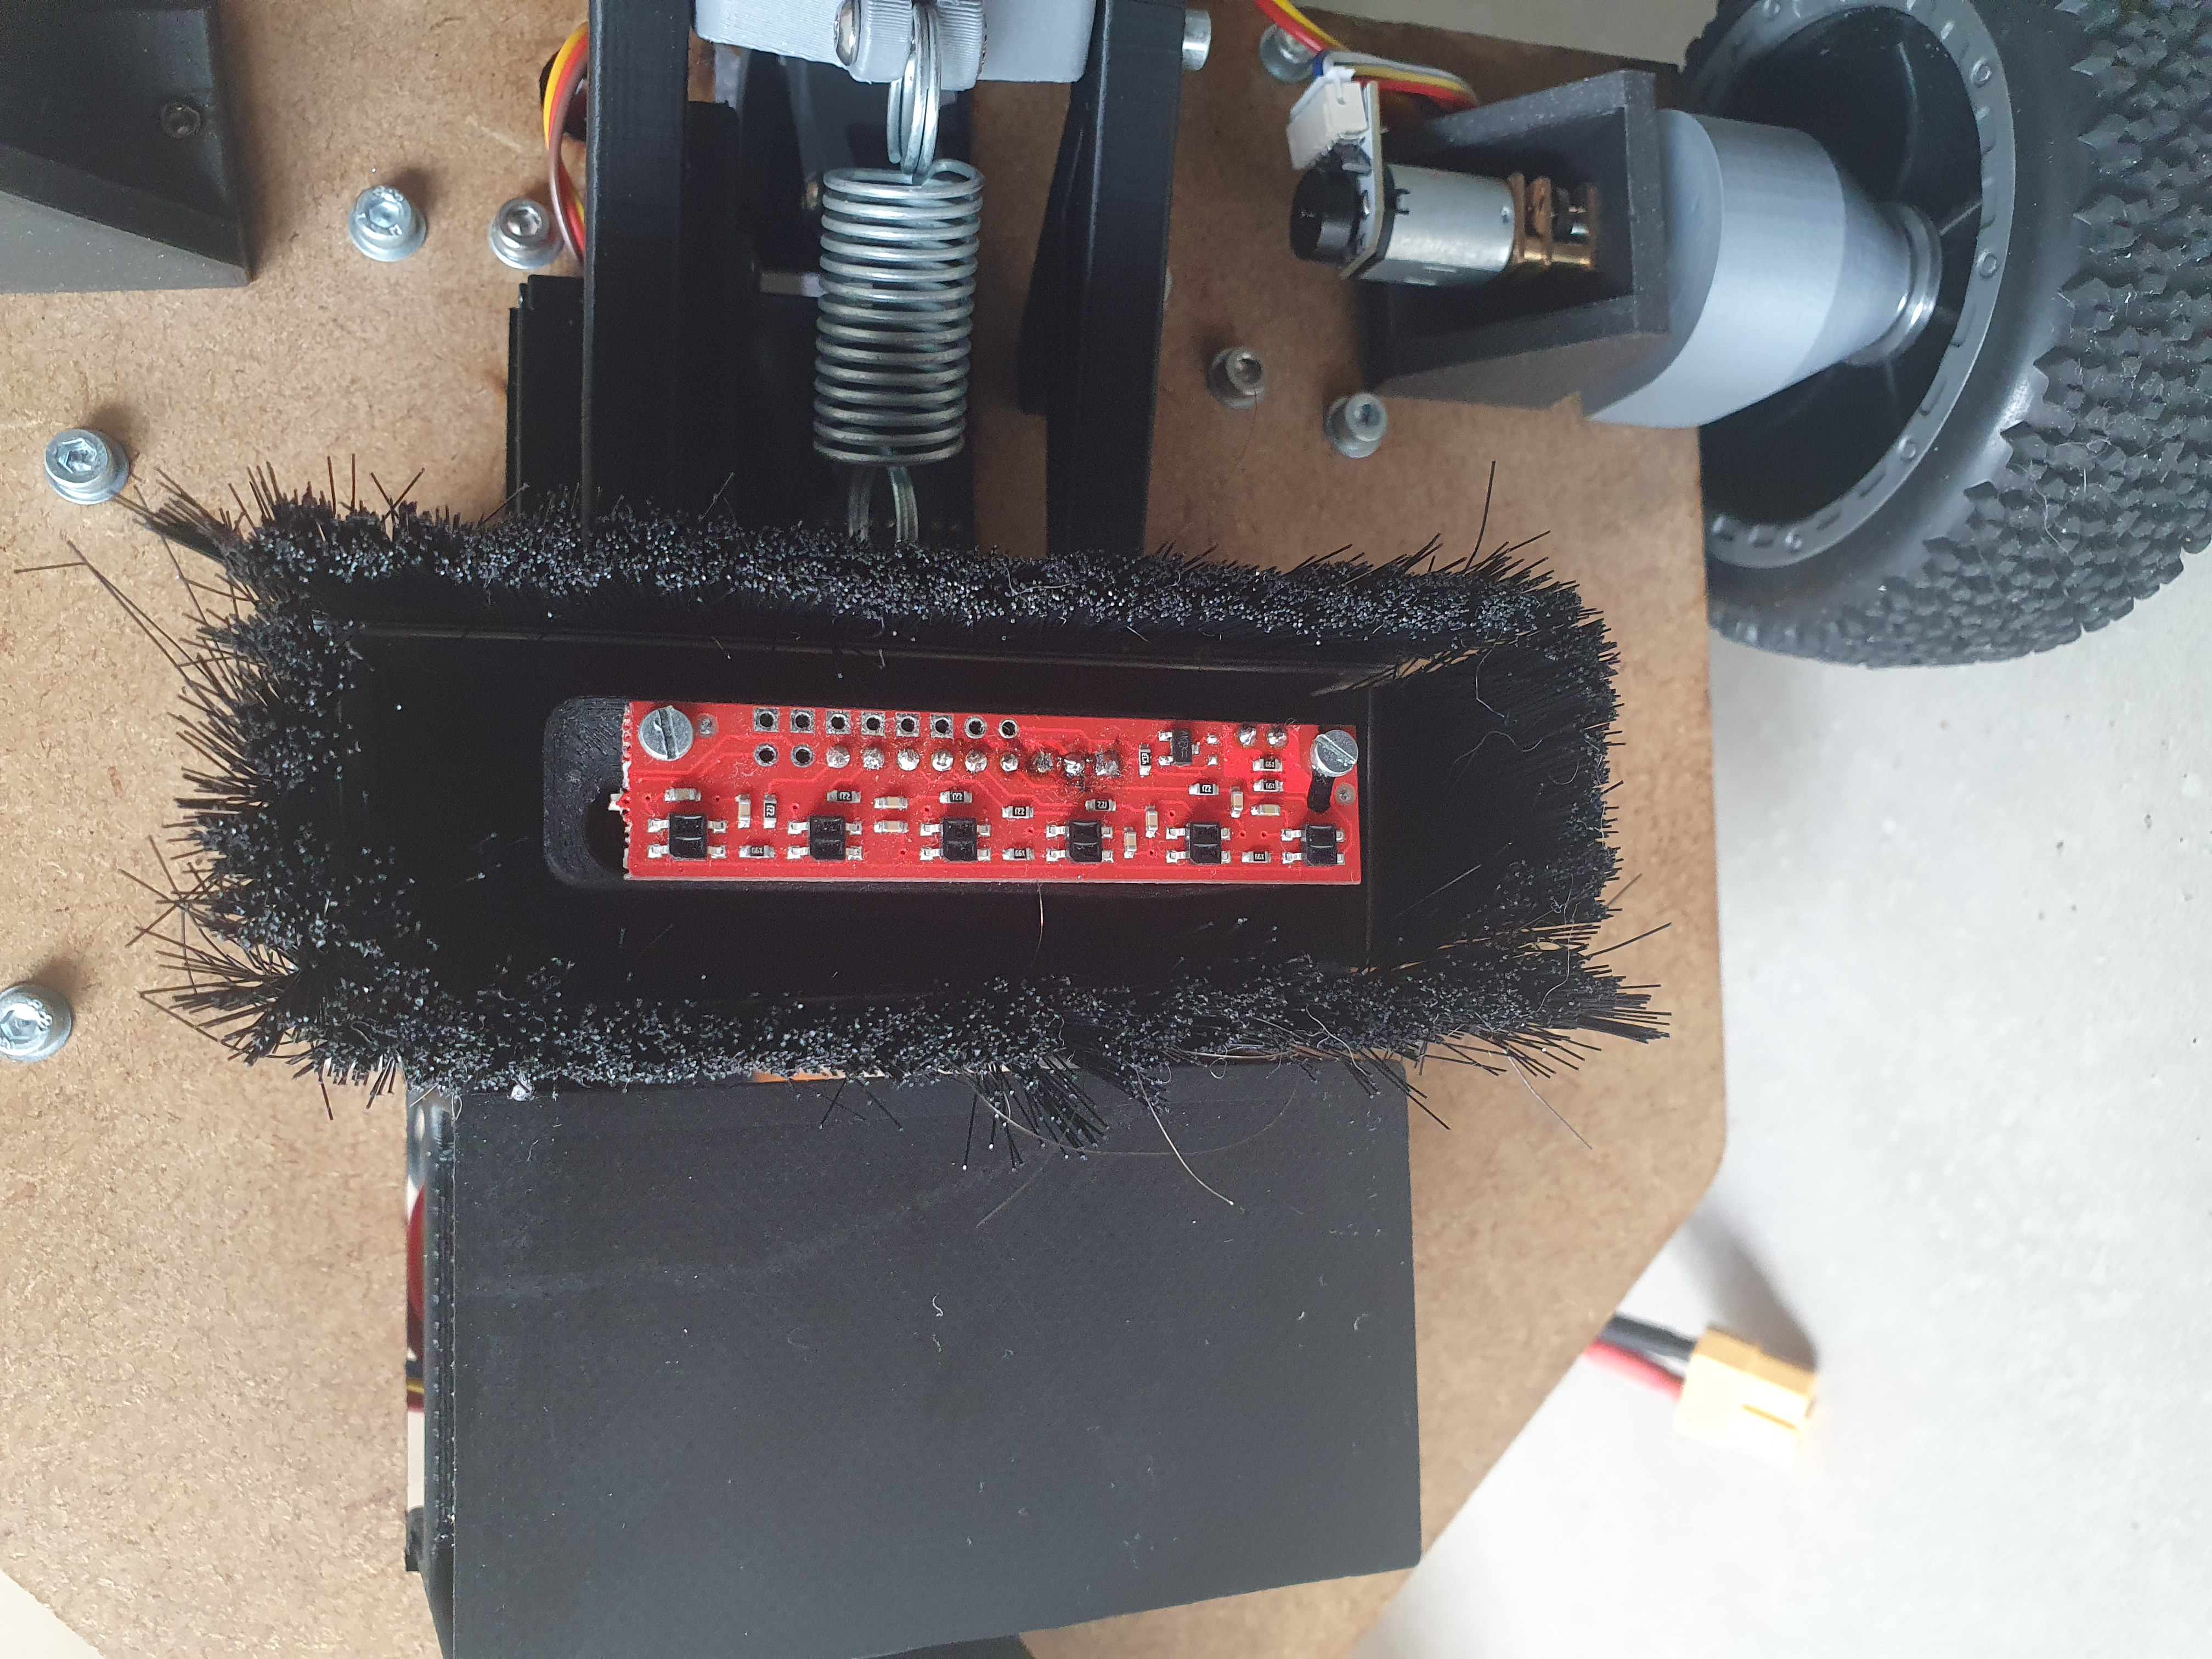
\includegraphics[width=0.5\textwidth ]{assets/MT/liniensensor-robi.jpg}
\caption{Liniensensor am Roboter}
\label{fig:linsen-robi}
\end{figure}


\newpage
%%%%%%%%%%%%%%%%%Epic 3%%%%%%%%%%%%%%%%%%%%%%%%%%%%%%%%%%%%%%%%%%%%%%%%%%%%%%%

\subsection{Bis zum nächsten Knoten fahren}

\subsubsection{Liniensensor}

Das Erkennen, ob der Roboter auf einem Wegpunkt steht oder nicht, wird ebenfalls mittels der Sensorwerten geprüft. Da beim Erreichen des Wegpunktes deutlich mehr Sensoren auf der weissen Oberfläche stehen, weichen die Werte der aktuellen Ticks stark den Sollwerten ab. Somit kann ein Wegpunkt klar identifiziert werden und der Roboter kann anhalten. Dies ist auf Abbildung \ref{fig:liniensensor_on_node} gezeigt.

\begin{figure}[H]
\centering
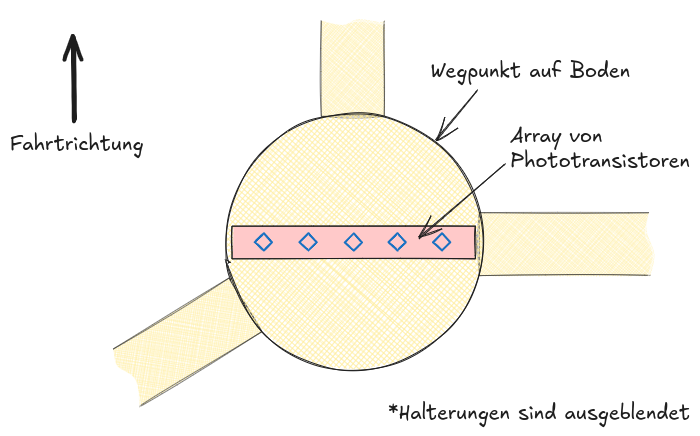
\includegraphics[width=0.5\textwidth ]{assets/ET/Liniensensor/linesensor_on_node.png}
\caption{Liniensensor auf Knoten}
\label{fig:liniensensor_on_node}
\end{figure}